\documentclass[10pt,a4paper]{report}

% Encoding and font
\usepackage[utf8]{inputenc}
\usepackage[T1]{fontenc}
\usepackage{lmodern}
\renewcommand{\familydefault}{\sfdefault}
\usepackage{textcomp} % symbols
\usepackage{xcolor}

% Page layout
\usepackage{geometry}
\geometry{
  a4paper,
  top=5cm,       % space for table header
  bottom=2.5cm,
  left=2.5cm,
  right=2.5cm,
  headheight=120pt
}
\usepackage{setspace}

% Headers and footers
\usepackage{fancyhdr}
\usepackage{lastpage}
\usepackage{appendix}
\pagestyle{fancy}
\fancyhf{}
\rfoot{\thepage}

% Tables
\usepackage{tabularx,booktabs,array,longtable,calc,xltabular}
\usepackage{multirow}
\usepackage{footnote}
\usepackage{datatool}
\usepackage{makecell}
\renewcommand{\arraystretch}{1.5}
\usepackage[table]{xcolor}

% Lists
\renewcommand{\labelenumii}{\arabic{enumi}.\arabic{enumii}}
\renewcommand{\labelenumiii}{\arabic{enumi}.\arabic{enumii}.\arabic{enumiii}}
\renewcommand{\labelenumiv}{\arabic{enumi}.\arabic{enumii}.\arabic{enumiii}.\arabic{enumiv}}

% Graphics
\usepackage{graphicx}
\makeatletter
\def\maxwidth{\ifdim\Gin@nat@width>\linewidth\linewidth\else\Gin@nat@width\fi}
\def\maxheight{\ifdim\Gin@nat@height>\textheight\textheight\else\Gin@nat@height\fi}
\setkeys{Gin}{width=\maxwidth,height=\maxheight,keepaspectratio}
\makeatother
\makeatletter
\def\fps@figure{htbp} % default figure placement
\makeatother
\usepackage{subcaption}

% Links
\usepackage{hyperref}
\hypersetup{
  hidelinks,
  pdfcreator={LaTeX via pandoc}
}
\urlstyle{same}

% Citations
\usepackage{apacite}
\bibliographystyle{apacite}

% Math
\usepackage{amsmath,amssymb}

% Misc
\usepackage{titlesec}
\usepackage{iftex}
\usepackage{subfiles}
\usepackage{pdflscape}
\usepackage[normalem]{ulem} % strikethrough support
\usepackage{ifthen}
\usepackage{glossaries-extra}
\setabbreviationstyle[acronym]{long-short}
\usepackage{datetime}
\ddmmyyyydate
\usepackage{mhchem}

% Optional enhancements
\IfFileExists{microtype.sty}{\usepackage{microtype}}{}
\IfFileExists{xurl.sty}{\usepackage{xurl}}{}
\IfFileExists{upquote.sty}{\usepackage{upquote}}{}

% Parskip handling
\makeatletter
\@ifundefined{KOMAClassName}{%
  \setlength{\parindent}{0pt}
  \setlength{\parskip}{6pt plus 2pt minus 1pt}
}{%
  \KOMAoptions{parskip=half}
}
\makeatother

% Custom commands
\newcommand{\todayISO}{%
  \the\year%
  \ifnum\month<10 0\fi\the\month%
  \ifnum\day<10 0\fi\the\day%
}%

\newcommand{\includesection}[1]{%
  \clearpage%
  \subfile{#1}%
}%

\newcommand{\iic}{%
  % I$^2$C%
  I\textsuperscript{2}C%
}%

\newcommand{\todo}[1]{%
  \colorbox{red}{\emph{#1}}%
}%

\renewcommand*\contentsname{Table of Contents:}
\setcounter{secnumdepth}{2}
\providecommand{\tightlist}{%
  \setlength{\itemsep}{0pt}\setlength{\parskip}{0pt}}

% Define header
\fancyhead[L]{%
  \renewcommand{\arraystretch}{1.4}
  \begin{tabularx}{\textwidth}{p{3cm}Xp{5cm}}
    \vspace{0mm}
    
\includegraphics[width=3cm]{media/stellar_space_logo.png}
     &
    \vspace{0mm}
    
\includegraphics[width=5.5cm]{media/inholland_logo.png}
     &
    \vspace{0mm}
    Document: Technical Report \newline
    Issue: 2.1 \newline
    Date: \today\newline
    Page: \thepage~of~\pageref{LastPage} \\
  \end{tabularx}%
}
% \fancyhead[L]{draft}

\fancypagestyle{noheader}{
  \fancyhf{}              % clear all header/footer
  \renewcommand{\headrulewidth}{0pt} % remove header line
  % \fancyfoot[L]{\thepage} % keep centered page number
}

\usepackage{tikz}
\usetikzlibrary{shapes.geometric, arrows, arrows.meta, positioning, calc, external}
\tikzexternalize[prefix=tikz/]

\tikzstyle{startstop} = [rectangle, rounded corners,
minimum width=3cm,
minimum height=1cm,
text centered,
draw=black,
fill=red!30]

\tikzstyle{io} = [trapezium,
trapezium stretches body=true, % A later addition
trapezium left angle=70,
trapezium right angle=110,
minimum width=3cm,
minimum height=1cm, text centered,
text width = 4cm,
draw=black, fill=blue!30]

\tikzstyle{sensor} = [trapezium,
trapezium stretches body=true, % A later addition
trapezium left angle=110,
trapezium right angle=70,
minimum width=3cm,
minimum height=1cm, text centered,
text width = 4cm,
draw=black, fill=green!30]

\tikzstyle{process} = [rectangle,
minimum width=4cm,
minimum height=1cm,
text centered,
text width=4cm,
draw=black,
fill=orange!30]

\tikzstyle{decision} = [diamond,
minimum width=4cm,
minimum height=1cm,
text centered,
draw=black,
fill=green!30]

\tikzstyle{arrow} = [thick,->,>=stealth]

\tikzstyle{pyprocess} = [rectangle,
minimum width=2cm,
minimum height=1cm,
text centered,
text width=3cm,
draw=black,
fill=orange!30]

\tikzstyle{pyvolume} = [rectangle,
% trapezium stretches body=true, % A later addition
% trapezium left angle=85,
% trapezium right angle=95,
minimum width=2cm,
minimum height=1cm,
text centered,
text width = 3cm,
draw=black, fill=blue!30]

\usepackage{tikz}
\usetikzlibrary{shapes.geometric, arrows, arrows.meta, positioning}

% Spring
\newcommand{\tikzspring}[2]{
    \draw[rotate=#1, thick, line join=bevel] (#2)
    -- +(0,0.25)
    -- +(0.05,0.5) -- +(0.15,0)
    -- +(0.25,0.5) -- +(0.35,0)
    -- +(0.45,0.5) -- +(0.55,0) -- +(0.6,0.25);

}

% Pressure Regulator
\tikzstyle{pressure regulator} = [rectangle,
minimum width=1cm,
minimum height=1cm,
append after command={
        \pgfextra{
            % \draw[help lines] (\tikzlastnode.center) ++(-1, -1) grid ++(2,2);
            \draw[thick, densely dashed] (\tikzlastnode.east) -- +(0.25,0.25) -- +(0.25,1) -- +(-0.75,1) -- +(-0.75,0);
            \draw[thick, fill=white] (\tikzlastnode.south west) -- +(1,0) -- +(1,1) -- +(0,1) -- +(0,0);
            \draw[->, thick, >=latex] (\tikzlastnode.west) -- (\tikzlastnode.east);
            \tikzspring{-90}{\tikzlastnode.south west}%
            \draw[->, thick, >=latex] (\tikzlastnode.south west) ++(-0.25, -0.175) -- +(1,-0.25);
        }
    }
]

% Orifice
\tikzstyle{orifice} = [rectangle,
minimum width=1cm,
minimum height=0.6cm,
append after command={
        \pgfextra{
            % \draw[help lines] (\tikzlastnode.center) ++(-1, -1) grid ++(2,2);
            \draw[thick] (\tikzlastnode.west) -- (\tikzlastnode.east);
            \draw[thick] (\tikzlastnode.north) ++(-0.38,0) arc (220:320:0.5);
            \draw[thick] (\tikzlastnode.south) ++(-0.38,0) arc (140:40:0.5);
            \draw[->, thick, >=latex] (\tikzlastnode.center) +(-0.2, -0.5) -- +(0.2,0.5);
        }
    }
]

% Volume
\tikzstyle{volume} = [rectangle,
minimum width=2cm,
minimum height=1cm,
append after command={
        \pgfextra{
            % \draw[help lines] (\tikzlastnode.center) ++(-1, -1) grid ++(2,2);
            \draw[thick, fill=white] (\tikzlastnode.south) ++(-0.5,0) -- ++(1,0) arc (-90:90:0.5) -- ++(-1,0) arc (90:270:0.5);
        }
    }
]

% Manual Valve
\tikzstyle{manual valve} = [rectangle,
minimum width=1cm,
minimum height=1cm,
append after command={
        \pgfextra{
            % \draw[help lines] (\tikzlastnode.center) ++(-1, -1) grid ++(2,2);
            \draw[thick, fill=white] (\tikzlastnode.south west) -- ++(1, 0) -- ++(0, 2) -- ++(-1, 0) -- ++(0, -2);
            \draw[thick] (\tikzlastnode.north west) -- (\tikzlastnode.north east);
            \draw[thick, <->, >=latex] (\tikzlastnode.west) -- (\tikzlastnode.east);
            \draw[thick] (\tikzlastnode.north west) ++(0, 0.5) -- ++(0.15, 0) ++(0, 0.1) -- ++(0, -0.2);
            \draw[thick] (\tikzlastnode.north east) ++(0, 0.5) -- ++(-0.15, 0) ++(0, 0.1) -- ++(0, -0.2);
            \draw[thick] (\tikzlastnode.south west) ++(0.05,0) -- ++(0, -0.5) ++(-0.05,0) -- ++(0.5,0) ++(-0.05,0) -- ++(0, 0.5);
        }
    }
]

% 5/2 Valve
\tikzstyle{5/2 valve} = [rectangle,
minimum width=1cm,
minimum height=0.5cm,
append after command={
        \pgfextra{
            % \draw[help lines] (\tikzlastnode.center) ++(-1, -1) grid ++(2,2);
            % Boxes
            \draw[thick, fill=white] (\tikzlastnode.west) ++(0, -0.5) -- ++(1, 0) -- ++(0, 2) -- ++(-1, 0) -- ++(0, -2);
            \draw[thick] (\tikzlastnode.west)  ++(0, 0.5)-- ++(1, 0);
            % Arrows
            \draw[thick, ->, >=latex] (\tikzlastnode.west) ++(0, 1) -- ++(1, 0.25);
            \draw[thick, ->, >=latex] (\tikzlastnode.east) ++(0, 0.25) -- ++(-1, 0);
            \draw[thick, ->, >=latex] (\tikzlastnode.west) -- ++(1, -0.25);
            \draw[thick, ->, >=latex] (\tikzlastnode.east) ++(0, 0.75) -- ++(-1, 0);
            % Plugs
            \draw[thick] (\tikzlastnode.west) ++(0, -0.25) -- ++(0.15, 0) ++(0, 0.1) -- ++(0, -0.2);
            \draw[thick] (\tikzlastnode.west) ++(0, 1.25) -- ++(0.15, 0) ++(0, 0.1) -- ++(0, -0.2);
            % Actuators
            \draw[thick] (\tikzlastnode.center) ++(-0.25,-0.5) -- ++(-0.25,-0.5) -- ++(0.5,0) -- ++(-0.25,0.5);
            \draw[thick] (\tikzlastnode.center) ++(-0.25,1.5) -- ++(-0.25,0.5) -- ++(0.5,0) -- ++(-0.25,-0.5);
            \draw[thick] (\tikzlastnode.west) ++(0, 1.5) -- ++(0, 1) -- ++(0.5, 0) -- ++(0, -1);
            \draw[thick] (\tikzlastnode.west) ++(0, 2.35) -- ++(0.5, -0.2);
        }
    }
]

% Volume
\tikzstyle{pressure sensor} = [rectangle,
minimum width=1cm,
minimum height=1cm,
append after command={
        \pgfextra{
            % \draw[help lines] (\tikzlastnode.center) ++(-1, -1) grid ++(2,2);
            % Air lines
            \draw[thick] (\tikzlastnode.west) -- ++(1, 0);
            \draw[thick] (\tikzlastnode.center) -- ++(0, 0.5);
            % Box
            \draw[thick, fill=white] (\tikzlastnode.north east) -- ++(0, 1) -- ++(-1, 0) -- ++(0, -1) -- ++(1, 0) -- ++(-1, 1);
            % P
            \draw[thick] (\tikzlastnode.center) ++(-0.3, 1) -- ++(0.1, 0) arc (90:-90:0.1) -- ++(-0.1, 0) ++ (0, 0.2) -- ++(0, -0.4);
            % n
            \draw[thick] (\tikzlastnode.center) ++(0.1, 1.1) -- ++(0,0.15) arc (180:0:0.15) -- ++(0,-0.15);
        }
    }
]

% Block
\tikzstyle{block} = [rectangle,
minimum width=1cm,
minimum height=1cm,
append after command={
        \pgfextra{
            % \draw[help lines] (\tikzlastnode.center) ++(-1, -1) grid ++(2,2);
            \draw[thick] (\tikzlastnode.west) -- ++(0.15, 0) ++(0, 0.1) -- ++(0, -0.2);
        }
    }
]

% \begin{tikzpicture}[node distance=2 cm]
%     \node[pressure regulator] (regulator1) {};
%     \node[manual valve, right of=regulator1] (valve1) {};

%     \node[orifice, right of=valve1] (orifice1) {};
%     \node[volume, right of=orifice1] (volume1) {};
%     \node[pressure sensor, right of=volume1] (sensor1) {};

%     \node[pressure regulator, right of=sensor1] (regulator2) {};

%     \node[5/2 valve, right of=regulator2,yshift=2cm, xshift=1cm] (purge valve) {};
%     \node[5/2 valve, right of=regulator2,yshift=-2cm, xshift=1cm] (normal valve) {};
%     \node[block, right of=purge valve, yshift=0.25cm, xshift=-1cm] (purge block) {};
%     \node[block, right of=normal valve, yshift=0.25cm, xshift=-1cm] (normal block) {};
%     \node[orifice, right of=purge valve, yshift=-0.25cm] (purge orifice) {};
%     \node[orifice, right of=normal valve, yshift=-0.25cm] (normal orifice) {};

%     % \draw[help lines] (-3, 0) grid (3,-6);
%     \draw [thick] (-1,0) -- (regulator1);
%     \draw [thick] (regulator1) -- (valve1);
%     \draw [thick] (valve1) -- (orifice1);
%     \draw [thick] (orifice1) -- (volume1);
%     \draw [thick] (volume1) -- (sensor1);
%     \draw [thick] (sensor1) -- (regulator2);
%     \draw [thick] (regulator2) -- ++(1.5,0) |- (purge valve);
%     \draw [thick] (regulator2) -- ++(1.5,0) |- (normal valve);
%     \draw [thick] (purge valve) ++(0.5, -0.25)-- (purge orifice);
%     \draw [thick] (normal valve) ++(0.5, -0.25)-- (normal orifice);
% \end{tikzpicture}%

% Air Supply
\newcommand{\airsupply}[2][airsupply]{
    \node (origin) {};

    \node[pressure regulator, right of=#2] (regulator1) {};
    \node[manual valve, right of=regulator1] (valve1) {};
    \node (#1) at (valve1) {};

    \draw [thick] (#2) -- (regulator1);
    \draw [thick] (regulator1) -- (valve1);
}

% CGG Equivalent
\newcommand{\aircgg}[2][aircgg]{
    \node (origin) {};

    \node[orifice, right of=#2] (orifice1) {};
    \node[volume, right of=orifice1] (volume1) {};
    \node[pressure sensor, right of=volume1] (sensor1) {};
    \node (#1) at (sensor1) {};

    \draw [thick] (#2) -- (orifice1);
    \draw [thick] (orifice1) -- (volume1);
    \draw [thick] (volume1) -- (sensor1);
}

% FC Equivalent
\newcommand{\airfc}[2][airfc]{
    \node (origin) {};

    \node[5/2 valve, right of=#2, yshift=2cm, xshift=1cm] (purge valve) {};
    \node[5/2 valve, right of=#2, yshift=-2cm, xshift=1cm] (normal valve) {};
    \node[block, right of=purge valve, yshift=0.25cm, xshift=-1cm] (purge block) {};
    \node[block, right of=normal valve, yshift=0.25cm, xshift=-1cm] (normal block) {};
    \node[orifice, right of=purge valve, yshift=-0.25cm] (purge orifice) {};
    \node[orifice, right of=normal valve, yshift=-0.25cm] (normal orifice) {};
    \node (#1) at (normal orifice) {};


    \draw [thick] (#2) -- ++(1.5,0) |- (purge valve);
    \draw [thick] (#2) -- ++(1.5,0) |- (normal valve);
    \draw [thick] (purge valve) ++(0.5, -0.25)-- (purge orifice);
    \draw [thick] (normal valve) ++(0.5, -0.25)-- (normal orifice);
}

\input{acronyms.tex}
\DTLnewdb{requirements}

\newcommand{\REQadd}[7]{
    \DTLnewrow{requirements}
    \DTLnewdbentry{requirements}{type}{#1}
    \DTLnewdbentry{requirements}{id}{#1-#2}
    \DTLnewdbentry{requirements}{level}{#3}
    \DTLnewdbentry{requirements}{statement}{#4}
    \DTLnewdbentry{requirements}{approach}{#5}
    \DTLnewdbentry{requirements}{verification}{#6}
    \DTLnewdbentry{requirements}{comment}{#7}
}

\newcommand{\REQ}[2]{%
    \DTLfetch{requirements}{id}{#1}{#2}%
}

\newcommand{\REQtable}[1]{

    \begin{tabularx}{\textwidth}{|r|X|}
        \hline
        \rowcolor{lightgray}
        \REQ{#1}{id}          & \REQ{#1}{statement}\hfill (\REQ{#1}{level}) \\%   & \REQ{#1}{level} \\
        \hline
        \cellcolor{lightgray}
        Proposed Approach     & \REQ{#1}{approach}                          \\
        \hline
        \cellcolor{lightgray}
        Verification Approach & \REQ{#1}{verification}                      \\
        \hline
        \cellcolor{lightgray}
        Comment               & \REQ{#1}{comment}                           \\
        \hline
    \end{tabularx}
}

\newcommand{\REQcategory}[1]{
    \DTLforeach[\DTLiseq{\type}{#1}]{requirements}
    {\type=type,\id=id}
    {
        \REQtable{\id}%
    }
}

\REQadd{Type}{ID}{Category}
{Requirement Statement}
{}
{}
{}

% Performance Requirements
\REQadd{PERF}{1}{M}
{The system shall be able to deliver 200 W continuous power}
{Ensure fuel cell meets power specifications from manufactures datasheet}
{Use wattmeter to verify}
{}

\REQadd{PERF}{2}{M}
{The system shall be able to supply loads varying from 140--220 W}
{Use a backup battery to provide power during peak loads}
{Use motor with propeller as variable load and wattmeter to verify}
{Variable load profile will be dependant on mission profile. Determine representative load profile with Wren Aerospace.}

% Operational Requirements
% -- How is it operated?
% “The product shall be designed to accept control of the viewing function from the ground segment”
% Runtime
% mission?
% Reports?
\REQadd{OP}{1}{D}
{The system should be able to deliver power for 13--16 hours}
{Choose a CGG size appropriate according to calculations}
{Use mass flow sensor to verify fuel consumption of fuel cell}
{}

\REQadd{OP}{2}{D} % Physical requirements?
{The mass of the power generation and feed system should not exceed 5 kg}
{Divide mass budget over subsystems and select parts that fit said mass budget}
{Use scale to verify}
{}

% Interface Requirements
% fuselage
% cgg (constant mdot)
% drone power
\REQadd{INT}{1}{D}
{The volume of the energy storage systems should not exceed 2.5 L}
{Design and select parts that fit in the given volume}
{Size measurement using calipers or other appropriate measurement devices}
{Verify with Wren Aerospace if this volume is also valid for the fuel cell system}

\REQadd{INT}{2}{D}
{The diameter of the energy storage system should not exceed 130 mm}
{Design and select parts that fit in the given diameter}
{Size measurement using calipers or other appropriate measurement devices}
{Verify with Wren Aerospace if this diameter is also valid for the fuel cell system}

\REQadd{INT}{3}{R}
{The fluid interface with the CGG shall have a maximum pressure of \textbf{XX} bar}
{Select parts compatible with this maximum pressure}
{Leakage test with compressed air}
{Exact value is dependant on buffer volume}

\REQadd{INT}{4}{R}
{The fluid interface with the CGG shall have a mass flow rate of \textbf{XX} g/min}
{Control fuel cell to use this mass flow rate of hydrogen using feedback control}
{Verify using mass flow sensor}
{Exact value dependant average power, battery size and CGG amount}

\REQadd{INT}{5}{R}
{The electrical interface with the flight controller shall have a voltage of \textbf{XX} V}
{Tune DC/DC converter to convert fuel cell output voltage to battery and flight controller voltage}
{Verify using mass voltmeter}
{Probably 6S LiPo voltage (18--25.2 V). Confirm with Wren}

% Environmental Requirements
% altitude
\REQadd{ENV}{1}{D}
{The system should be able to operate at altitudes up to 3 km}
{Verify fuel cell performance at appropriate atmospheric conditions}
{}
{Split up in temperature, pressure and oxygen content requirements?}

\REQadd{ENV}{2}{D}
{The system should be able to operate at speeds up to 21 m/s}
{Verify fuel cell performance at appropriate atmospheric conditions}
{}
{Translate to spec demands for fuel cell}


% Safety Requirements
% h2
\REQadd{SAFE}{1}{R}
{The system shall have a total hydrogen leakage lower than \textbf{XX}}
{Design using COTS components rated for appropriate pressure}
{Verify with leakage test}
{}

\input{researchquestions.tex}
% \input{workpackages.tex}

% Define the Title Page
\title{\textbf{Project SHARP- Power Generation and Delivery System} \\ \vspace{1cm}
\textbf{Technical Report}}
\author{Emil Boot}
\date{\today}

\begin{document}
% Import sections from the sections folder
\input{sections/titlepage.tex}
% Change record section
% File: sections/change_record.tex

\chapter*{Change record}
\begin{table}[htp]
  \centering
  \renewcommand{\arraystretch}{1.2} % row height
  \begin{tabularx}{\textwidth}{|l|l|l|l|X|}
    \hline
    Issue & Date                     & Total pages & Page(s) affected      & Description of change                                                          \\
    \hline
    0.0   & \formatdate{24}{2}{2026} & 11          & 0--11                 & Adapt Initial Template                                                         \\
    \hline
    0.1   & \formatdate{16}{3}{2026} & 27          & 3--15, 18--21, 24--27 & Added preliminary chapters 1, 2 \& 5                                           \\
    \hline
    0.2   & \formatdate{20}{4}{2026} & 30          & 13--16, 21--28        & Continued Chapter 5, Finished requirements                                     \\
    \hline
    0.3   & \formatdate{29}{4}{2026} & 40          & 18--21, 24, 32        & Added Simulation Ch. 2.3                                                       \\
    \hline
    0.4   & \formatdate{12}{5}{2026} & 46          & 19--38                & Reorganised Chapters, Added Ch. 4 \& 6                                         \\
    \hline
    0.5   & \formatdate{15}{5}{2026} & 49          & 33--38                & Added Ch. 5.3                                                                  \\
    \hline
    1.0   & \formatdate{15}{5}{2026} & 49          & all                   & Reviewed and finalised all chapters                                            \\
    \hline
    1.1   & \formatdate{28}{5}{2026} & 49          & 3, 12, 37, 43--44     & Added Abstract, mission scenario, h2 results                                   \\
    \hline
    2.0   & \formatdate{30}{5}{2026} & 68          & 2, 34, 45--56, 60--67 & Added Preface, requirement validation, conclusion, recommendations, appendices \\
    \hline
  \end{tabularx}
\end{table}

\newpage


\chapter*{Preface}
\addcontentsline{toc}{chapter}{Preface}
TBD

\chapter*{Abstract}
\addcontentsline{toc}{chapter}{Abstract}
This thesis seeks the answer to the research question: `To what extent is a hydrogen fuel cell based power generation and feed system that integrates a Solid Flow's cool gas generator and Stellar Space Industries' flow control unit feasible for extending the mission time for UAV's'

This document covers the design process of this power generation and feed system. The system will use hydrogen from a Cool Gas Generator (CGG) that stores hydrogen as solid \ce{NaBH4} and produces a constant stream of hydrogen gas. This hydrogen gas is then fed to a Fuel Cell to generate power. A battery is used as a power buffer to support varying loads while consuming a constant amount of hydrogen. The Fuel Cell periodically cleans excess water from its fuel intake by performing purge events during which it uses hydrogen at an increased rate. To make this compatible with the constant flow of the CGG a buffer volume is used to store a small amount of hydrogen for this purpose. A Flow Control Unit (FCU) is used to provide hydrogen from this buffer to the Fuel Cell at the correct pressure.

To verify the design, a test bench has been developed that includes a Fuel Cell, CGG flow equivalent, FCU, battery and motor and propeller as representative load, as well as numerous sensors to document the system behaviour. Preliminary results of this test bench are presented in this thesis which suggest that the designed power generation and feed system is capable of more than doubling the mission time of a UAV. However, due to neither a CGG or a hydrogen tank being available during the project, final tests using this test bench are still waiting to be performed.

% Table of Contents:
\newpage
{\large \tableofcontents}
\newpage
\listoffigures
\addcontentsline{toc}{chapter}{List of Figures}
\listoftables
\addcontentsline{toc}{chapter}{List of Tables}

\chapter{Introduction}%
\label{chap:intro}
TBD
\newpage

\input{project plan sections/01_project_background.tex}
\section{Project Results}
For Stellar Space Industries, the primary goal for SHARP is to test and apply their FCU in a real world scenario and thus advance the FCU's technology readiness level (TRL) from 4 to 6. In addition to this, they aim to find a secondary market for their FCU in hydrogen based aviation compared to electric propulsion for satellites. Solid Flow has the same goals for their hydrogen CGG.
The goal of SHARP-PS is to integrate the FCU and CGG and demonstrate the technologies and their compatibility in a relevant environment.

The relevant evnironment for the SHARP-PS project will be a hydrogen fuel cell that delivers power to an unmanned areal vehicle (UAV). The results of the SHARP-PS project will be the following:

\begin{itemize}
    \item The design for a power generation and feed system that is integrated into a UAV.
    \item A test bench setup that validates the performance of this power generation and feed system.
    \item A research report that documents the design process and test results and assesses the feasibility of using this power system in UAV's.
\end{itemize}

If allowed by time, a UAV with the integrated power generation and feed system may be an additional result of the SHARP-PS project. This will be described in more detail in section 4 Scope.

% The relevant environment for the SHARP-PS project will be a fuel cell that delivers power to a motor and propeller system. Results of tests performed in this environment will be directly applicable to hydrogen based aviation projects. The result of the SHARP-PS project will be a test bench setup that includes this fuel cell and motor-propeller system and the integrated FCU and CGG hydrogen supply. This test bench setup shall be easily adaptable to be integrated into an unmanned areal vehicle (UAV). The project result of SHARP-PS shall meet the following requirements:

Requirements for the UAV are not described in this document. These are dependent on the mission scenario for the UAV which, as of the writing of this document, has not yet been determined. This mission scenario will be determined by Stellar Space Industries as soon as possible, after which the requirements for the UAV will be constructed. Requirements for the other results of the SHARP-PS project are as follows:

\begin{itemize}
    \item Stellar Space Industries' FCU shall be included in the system.
    \item Solid Flow's hydrogen CGG shall be included in the system.
    \item A fuel cell shall be used to generate electricity from hydrogen.
    \item The system shall function without external power supply.
    \item The power density (power output over system weight) of the system must be the same or higher than that of state-off-the-art UAV power systems.
    \item Test results will be recorded and presented in a research report that is in accordance with `Report writing for readers with little time'~\cite{EllingAndeweg2012}
    \item The research report shall answer the following research question: `To what extent is a hydrogen fuel cell based power generation and feed system that integrates a Solid Flow's cool gas generator and Stellar Space Industries' flow control unit feasible for extending the mission time for UAV's'
\end{itemize}
\newpage

The aforementioned research question will be subdivided into the following sub research questions:

% \textbf{Sub Research Questions}\\
\begin{enumerate}
    \DTLforeach{researchquestions}{
    \id=id%
    }{
    \renewcommand{\labelenumi}{\id}
    \item{\RQ{\id}{long}}
          }
\end{enumerate}

These research questions have been arranged into a research matrix where they have been assigned a research method and is specified what instruments or tools are used and what the output is of each research question. This research matrix is shown in Appendix~\ref{app:Research Matrix}.

\newpage




\newpage

\section{Research}%
\label{sec:research}

\emph{This section contains literature research that applies to the SHARP-PS project. The workings of fuel cells are explained in detail. A comparison is made that evaluates the effectiveness of energy storage as hydrogen tanks versus batteries. Several papers are described of other projects that are similar to the SHARP project. The results and design choices made during these projects might be of interest during the SHARP-PS project.}

\subsection{PEM Fuel Cells}
Fuel cells are a technology that produce electricity from gases directly without combustion. There are many different types of fuel cells that run on different types of gases. These include solid oxide fuel cells (SOFC), direct methanol fuel cells (DMFC) and proton exchange membrane fuel cells (PEMFC). The PEMFC is used widely as it has a relatively high power density and a low operating temperature \cite{Kim:NaBH}. These properties are especially beneficial for UAV power systems.

The book \emph{Fuel Cells} by \citeA{revankar-2016} describes the working of the PEMFC in great detail. The PEMFC works by letting hydrogen undergo a series of electrochemical reactions. At the anode the hydrogen is split into protons ($H^+$) and electrons ($e^-$). The protons pass through the Proton Exchange Membrane (PEM), but the electrons can't pass through this membrane and must follow the external electrical circuit. The protons and electrons both arrive at the cathode where they react with oxygen to form water. This process is shown in a schematic diagram in figure~\ref{fig:fuelcell single}.

% Introduce Stack?
As a single fuel cell typically produces 0.7 volts, multiple cells are often connected in a stack. The membrane electrode assembly (MEA) is sandwiched between two conducting plates that have integrated flow channels for the hydrogen, oxygen and water. A schematic overview of a stack including three cells is provided in figure~\ref{fig:fuelcell stack}.

\begin{figure}[htp]
    \begin{subfigure}{0.5\textwidth}
        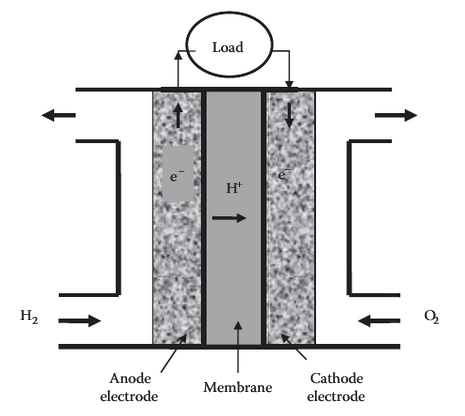
\includegraphics[width=0.9\linewidth, height=8cm]{media/FuelCell.png}
        \caption{Single Fuel Cell}
        \label{fig:fuelcell single}
    \end{subfigure}
    \begin{subfigure}{0.5\textwidth}
        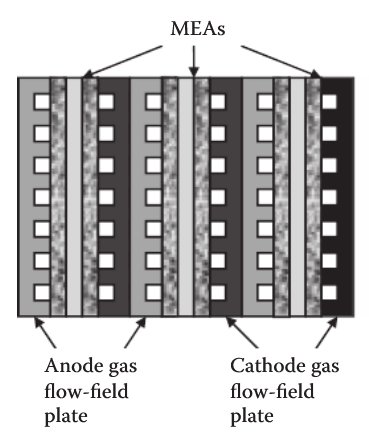
\includegraphics[width=0.9\linewidth, height=7cm]{media/FuelCellStack.png}
        \caption{Fuel Cell Stack}
        \label{fig:fuelcell stack}
    \end{subfigure}
    \caption{Fuel Cell Schematic Diagrams}
    \label{fig:fuelcell overview}
\end{figure}

As visible in figure~\ref{fig:fuelcell single}, hydrogen not only flows into the anode side of the fuel cell, but also out of that side. Simply leaving this side open to the air not only wastes a lot of unused hydrogen but also poses a major safety risk~\cite{Li:circulation}. If this side of the anode is simply blocked off, impurities in the hydrogen and liquid water generated by the reaction accumulate over time, blocking the hydrogen supply. Instead, a purge valve can be installed that periodically purges the anode side and removes gas impurities and excess water. While this design is simple it still leads to periodic voltage drops and reduced power output.
\citeauthor{Li:circulation} introduces several circulation mechanisms to prevent this and enhance both safety and fuel utilisation. These circulation mechanisms include recirculation pumps, ejector valves or a combination of both. However both of these systems only become efficient for fuel cells operating above 80 kW, which is orders of magnitude higher than required for the fuel cell in this project.

\subsection{Comparison of Energy Storage Methods}
The SHARP project aims to extend the flight time of drones and possibly small aircraft in the future. It aims to do this by providing an alternative energy source that is more weight efficient than current solutions. To keep track of the progress and improvements that are made by the SHARP project the energy density of current solutions are analysed.

Different aspects of energy density play a role in aviation systems. Most important is the gravimetric energy density, which refers to the amount of stored energy per unit mass. For hydrogen this is 142 MJ/kg, nearly three times that of kerosene at 50 MJ/kg. However, volumetric energy density also plays a role and it refers to the amount of stored energy per unit volume. For hydrogen at atmospheric pressure this is only 0.01 MJ/L while for kerosene this is much higher at 35 MJ/L. For this reason, hydrogen is often stored in pressurised tanks or as a cryogenic liquid. This significantly increases the volumetric energy density as can be seen in table~\ref{tab:fuels}.

\begin{table}[htp]
    \centering
    \begin{tabularx}{0.75\textwidth}{X r r}
        \toprule
        \textbf{Fuel}      & \textbf{Gravimetric [MJ/kg]} & \textbf{Volumetric [MJ/L]} \\
        \midrule
        Gasoline           & 46                           & 34                         \\
        Kerosene           & 50                           & 35                         \\
        Hydrogen (1 bar)   & 142                          & 0.01                       \\
        Hydrogen (350 bar) & 142                          & 3                          \\
        Hydrogen (700 bar) & 142                          & 5                          \\
        Hydrogen (liquid)  & 142                          & 8.5                        \\
        \bottomrule
    \end{tabularx}
    \caption{Energy density of fuels}
    \label{tab:fuels}
\end{table}

The gravimetric energy density of hydrogen itself may be very high, however pressurised storage vessels are quite heavy and thus their weight cannot be neglected. Generally, the hydrogen stored in a pressurised cylinder only contributes 2 to 5\% of the total weight of the cylinder. This weight percentage is dependant on the cylinder shape and size. Intelligent Energy, a fuel cell supplier, has provided an overview of currently available hydrogen storage cylinders of different sizes from different suppliers~\cite{IE:cylinders}. This is shown in figure~\ref{fig:IE cylinders}.

\begin{figure}[htp]
    \centering
    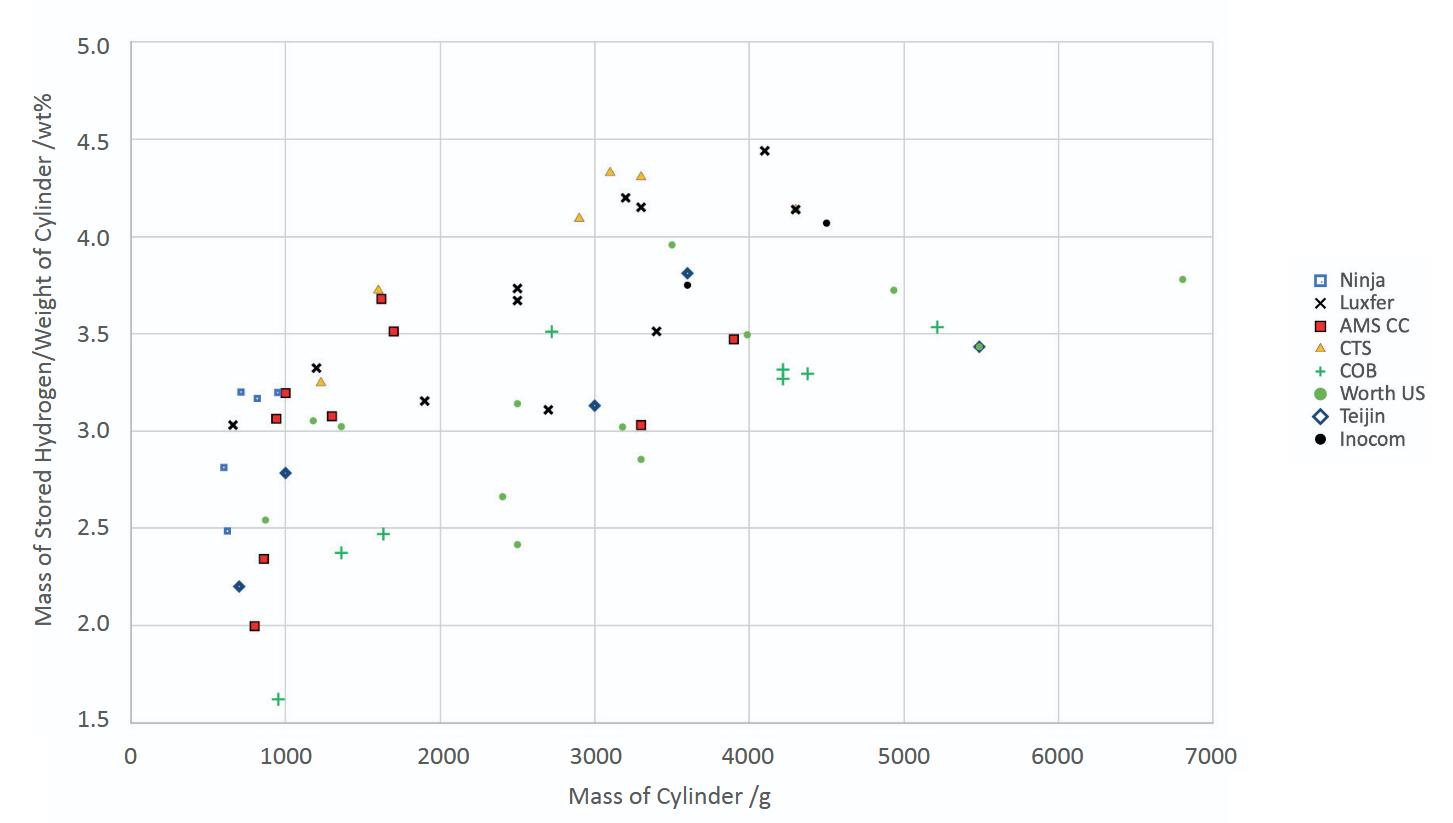
\includegraphics[width=0.75\textwidth]{media/IE_cylinders.png}

    \caption{Gravimetric Energy Density comparison of hydrogen Cylinders by Intelligent Energy}
    \label{fig:IE cylinders}
\end{figure}

Hydrogen cylinders can now be compared with LiPo batteries, which are a popular energy storage solution for UAVs. From figure~\ref{fig:IE cylinders} it is clear that hydrogen cylinders become more weight efficient at larger sizes. LiPo batteries also come in different shapes and sizes, however they do not share this increase in efficiency with hydrogen cylinders. A comparison has been made the energy density of different systems at different storage sizes, this is shown in figure~\ref{fig:Energy Storage}. The comparison includes some of the smaller Hydrogen cylinders from AMS CC from the comparison by Intelligent Energy, as well as some even smaller hydrogen tanks by MyH2. Several LiPo batteries have been included as well as batteries of some popular drones by DJI. A fuel cell efficiency of 40\% was assumed when determining the energy capacity of the hydrogen cylinders.

\begin{figure}[htp]
    \centering
    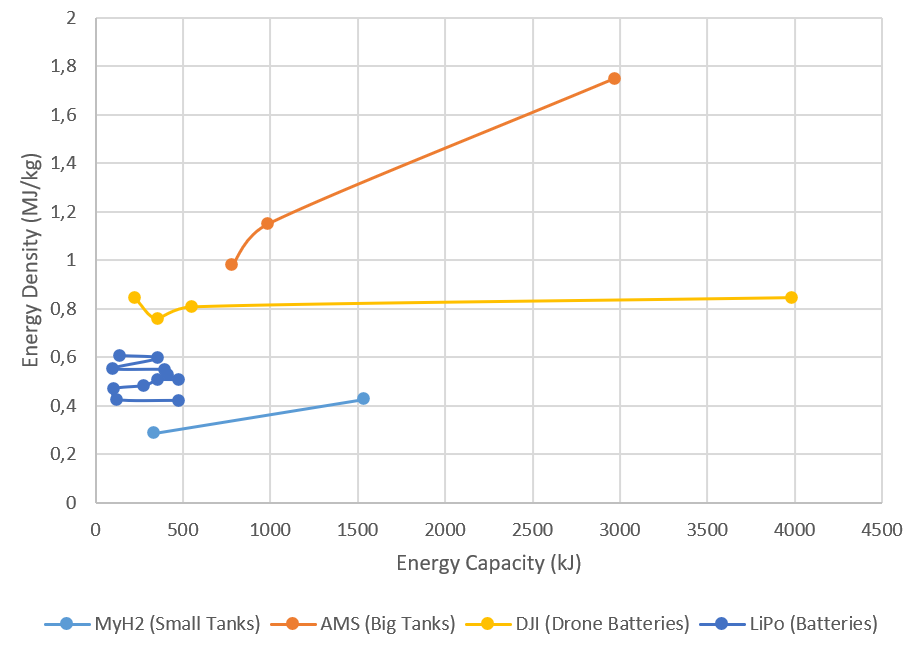
\includegraphics[width=0.75\textwidth]{media/Energy_Storage.png}
    \caption{Gravimetric Energy Density comparison of different energy storage solutions}
    \label{fig:Energy Storage}
\end{figure}

The goal of this comparison is to find a break-even point where hydrogen cylinders become more efficient than batteries. Unfortunately, figure~\ref{fig:Energy Storage} does not give an exact point, however the first hydrogen cylinder that is more efficient than batteries has an energy capacity of 780 kJ, above this point hydrogen cylinders are more efficient than batteries. Noteworthy is that this is more than double the capacity of the DJI Inspire, a large consumer drone, at 350 kJ. This means that for doubling the flight time of this drone, it would require less mass to just add an extra battery than to replace its battery with a hydrogen system.

Figure~\ref{fig:Energy Storage} compares the gravimetric energy density of energy storage solutions,  but ignores the weight of the system required to actually retrieve this energy. Figure~\ref{fig:Energy Storage} was made specifically for the context of the SHARP project where hydrogen is generated at a using a CGG. In order to decouple the constant rate of energy generation from the fluctuating energy consumption of the drone an energy buffer is required. Figure~\ref{fig:Energy Storage} allows comparison for using a battery or hydrogen cylinder as this buffer. In this specific case, the fuel cell system is required regardless of whether the energy buffer is implemented as a battery or as a hydrogen tank, and thus its weight does not play a role in their comparison.

However, when comparing using hydrogen cylinders with a fuel cell to using batteries without a fuel cell, the weight of the fuel cell must also be considered.



\subsection{Hydrogen Drones}
Several studies have been performed on the feasibility of hydrogen drones using PEMFCs. One notable example is \citeA{NLR:HYDRA}, their HYDRA project produced an 8kg hexacopter running on an 800W fuel cell for the Royal Netherlands Aerospace Centre (NLR). Their HYDRA-1B power system achieved and energy density of about 0.36 kWh/kg which is higher than that of commercial LiPo batteries at about 0.2 kWh/kg and still has significant potential for improvement. Their paper on the HYDRA project goes into detail about the drone design and part selection as well as hydrogen safety. This may provide a starting point for the design of the SHARP-PS project as the target scale of the drone and power system are similar.

Another example is \citeA{Nederdrone} who produced a Vertical Take-Off and Landing (VTOL) UAV called the Nederdrone, which runs on the same 800W fuel cell. In addition to stating the processes of fuel cell selection and drone design, they also go into detail about their hybrid power system using batteries to supply additional power during peak load.

Notable is that both systems use the same fuel cell by Intelligent Energy in combination with backup batteries. In addition to that, both projects are recent projects executed in the Netherlands, which may enable easy consultation if necessary. Stellar Space Industries has contacted NLR, who have expressed interest in the SHARP project.

\newpage


\chapter{Requirements}%
\label{sec:requiements}

\emph{From the mission scenario presented by Wren Aerospace et al. (discussed in section~\ref{sec:mission_scenario}) a set of system requirements is derived. From this mission scenario the system functions are formulated, which are decomposed into subfunctions. The system requirements are then allocated to these system functions.}
\newpage

% System level Requirements
\section{User Level Requirements}

% user reqs
The user requirements defined by Stellar Space Industries, Solid Flow and Wren Aerospace are summarised below:
\begin{itemize}
    \item The system shall include SSIs FCU
    \item The system shall include SolidFlows CGG
    \item The system shall integrate with WrenAerospaces UAV
    \item The system shall produce electricity from hydrogen
          % \item Shall function without external psu %(covered by wren)
    \item The system shall have a power density greater than or comparable to UAVs %(covered by wren)
\end{itemize}

\section{System Level Requirements}
These user requirements are translated to system requirements in a structured manner. Each requirement will adhere to the following structure:

\REQtable{Type-ID}

\begin{itemize}
    \item Type: Type of requirement e.g. Performance Requirement (PERF)
    \item ID: Sl no.
    \item Requirement Statement --- a brief and unambiguous representation of the requirement
    \item Requirement Approach --- provides information on the scope and how the requirement could be achieved
    \item Verification Approach --- presents plan on how the specified requirement will be verified
    \item Category: Mandatory (M), Desirable (D), Optional (O)
\end{itemize}

% Requirements from Wren Aerospace
% \begin{itemize}
%       % Wren email
%       \item The system shall be able to deliver 200 W continuous power
%       \item The system shall be able to supply loads varying from 140--220 W
%       \item The system shall be able to deliver power for 13--16 hours
%       \item The mass of the energy storage system should not exceed 2.8 kg
%       \item The mass of the fuel cell system should not exceed 2.2 kg
%       \item The volume of the energy storage system should not exceed 2.5 L
%       \item the diameter of the energy storage system should not exceed 130 mm
%             % Volume and diameter also applicable for fuel cell system?
%       \item The system should be able to operate at altitudes up to 3 km
%       \item The system should be able to operate at speeds up to 21 m/s

% \end{itemize}

\clearpage

\subsection*{Performance Requirements}
\REQcategory{PERF}

\subsection*{Operational Requirements}
\REQcategory{OP}

\subsection*{Interface Requirements}
\REQcategory{INT}

\subsection*{Environmental Requirements}
\REQcategory{ENV}

\subsection*{Safety Requirements}
\REQcategory{SAFE}

% Reliability and Maintainability?


% SRS Document:

% Temperature range
% Humidity range
% FC efficiency
% backup battery mission
% CGG reqs?
% Drone reqs?
\newpage

% \subsubsection{Functional Decomposition}
% Subsystem level Requirements
% \subsection{Subsystem Level Requirements}


% Based on the mission scenario, a list has been constructed of functions that the system needs to be able to fulfil. Each of these functions will represent a subsystem of the power generation and delivery system. The identified subsystems are as follows:
% \begin{itemize}
%       \item Manage Hydrogen Supply %(FCU)
%       \item Hydrogen Conversion %(FC)
%       \item Intermediate Energy Storage %(LiPo, H2 buffer)
%       \item Electricity Conditioning %(DC/DC, Diode?, LiPo charger?)
%       \item Monitoring and Control %(microcontroller)
%             % \item Ensure Safety
% \end{itemize}

% The requirements for each subsystem will be discussed in the following sections. Each subsystem level requirement is either a system level requirement that has been allocated to a specific subsystem, or a requirement derived from a system level requirement.


% Functional Decomposition % Functional requirements

% Base function: supply electric power
% \\Subfunctions:

% \begin{itemize}
%       \item Manage Hydrogen Supply (FCU)
%             \begin{itemize}
%                   \item Receive Hydrogen from CGG
%                   \item Regulate Hydrogen pressure and flow
%             \end{itemize}
%       \item Hydrogen Conversion (FC)
%             \begin{itemize}
%                   \item Supply hydrogen to fuel cell
%                   \item Generate electrical power using fuel cell
%                   \item Remove fuel cell byproducts
%             \end{itemize}
%       \item Intermediate Energy Storage (LiPo, H2 buffer)
%             \begin{itemize}
%                   \item Reduce power demand during peak loads
%                   \item Store excess energy produced by CGG
%                   \item Monitor energy buffer level
%                   \item Prevent overcharge/overdischarge of energy buffer
%                   \item Store Energy for emergency landing
%             \end{itemize}
%       \item Electricity Conditioning (DC/DC, Diode?, LiPo charger?)
%             \begin{itemize}
%                   \item Regulate output voltage
%                   \item Regulate output current
%                   \item Deliver power to host (UAV)
%                   \item Protect fuel cell from back current
%                   \item Synchronise fuel cell and other power sources
%             \end{itemize}
%       \item Monitoring and Control (microcontroller)
%             \begin{itemize}
%                   \item Monitor hydrogen pressure and flow
%                   \item Monitor fuel cell performance
%                   \item Monitor energy storage level
%                   \item Execute control algorithms
%                   \item Start CGG when required
%                   \item Communicate system status to host (UAV)
%             \end{itemize}
%       \item Ensure Safety
%             \begin{itemize}
%                   \item Prevent fuel cell overload
%                   \item Prevent pressure build-up
%                   \item Prevent thermal runaway
%                   \item Execute emergency shutdown
%             \end{itemize}
% \end{itemize}

% \subsubsection{Hydrogen Supply}
% \subsubsection{Hydrogen Conversion}
% \subsubsection{Intermediate Energy Storage}
% \subsubsection{Electricity Conditioning}
% \subsubsection{Monitoring and Control}
% \subsubsection{Safety}


\newpage

% \chapter{Concept Design}%
% \label{chap:concept design}%
% \emph{In this chapter different system architectures are proposed for the hydrogen based power generation and feed system. The different architectures are then compared using a trade-off table on the basis of which one architecture is selected.}
% \newpage

% \section{Description of System Architectures}
% A morphological chart has been constructed to compare different implementations of the required system functions. This chart is shown in table~\ref{tab:morphological chart}.
% \begin{table}[htp]
%     \begin{tabularx}{\textwidth}{|l|>{\centering\arraybackslash}X|>{\centering\arraybackslash}X|>{\centering\arraybackslash}X|}
%         \hline
%         \textbf{System Functions} & \textbf{Option 1}        & \textbf{Option 2} & \textbf{Option 3} \\
%         \hline
%         Fuel Cell Throttle        & Hydrogen Flow Controller & Current Limiter   & Relay             \\
%         \hline
%         Energy Storage            & Battery                  & Hydrogen Tank     &                   \\
%         \hline
%         Throttle Control          & On-Off                   & PID               & Fuzzy Logic       \\
%         \hline
%     \end{tabularx}
%     \caption{Morphological chart of the Power Generation and Feed System Architectures}
%     \label{tab:morphological chart}
% \end{table}

% % Changes with respect to Architecture 1 are highlighted in green.
% \newcommand{\new}[1]{\cellcolor{green!80!yellow!50}\emph{#1}}
% \begin{table}[htp]
%     \begin{tabularx}{\textwidth}{l>{\centering\arraybackslash}X>{\centering\arraybackslash}X>{\centering\arraybackslash}X}
%         \toprule
%                                     & \textbf{Architecture 1}  & \textbf{Architecture 2} & \textbf{Architecture 3} \\
%         \midrule
%         \textbf{Fuel Cell Throttle} & Hydrogen Flow Controller & Relay                   & Current Limiter         \\
%         \textbf{Energy Storage}     & Hydrogen Tank            & Battery                 & Battery                 \\
%         \textbf{Throttle Control}   & Fuzzy Logic              & On-Off                  & PID                     \\
%         \midrule
%         \textbf{Advantages}         & Simple Electronics       & Simple Control System   & Stable Power Delivery   \\
%         \textbf{Disadvantages}      & Heavy at small scale     & Power Spikes            & Complex Electronics     \\
%                                     & No Backup Battery        &                         &                         \\
%         \bottomrule
%     \end{tabularx}
%     \caption{Proposed System Architectures}
%     \label{tab:architectures}
% \end{table}

% \section{Architecture Trade-Off and Selection}

% \textbf{arch 2:}
% \\weight of 1L tank vs weight of pressure regulator

% \textbf{arch 3:}
% \\max switching frequency of fc, DC/DC
% \\effectiveness of smoothing capacitor

% \textbf{arch 4:}
% \\required flexibility
% \\weight efficiency of small vs large cggs

% \textbf{arch 5/6:}
% \\required flexibility
% \\required mission time
% \\required energy for (emergency) landing

% \textbf{\Large{CHATGPT VERSION}}

\chapter{Concept Design}
\label{chap:concept design}

\emph{This chapter presents the conceptual design process of the hydrogen-based power generation and feed system. Different system architectures are generated using a morphological analysis method and subsequently evaluated using a trade-off study. Based on this evaluation, the most suitable architecture is selected for further development.}

\newpage

\section{System Objectives and Functional Requirements}

The purpose of the power generation and feed system is to provide reliable electrical power using hydrogen generated from Solid Flow's cool gas generator. The generated hydrogen is supplied to a fuel cell, which converts the chemical energy into electrical energy.

The conceptual design of the system is driven by the following primary objectives:

\begin{itemize}
    \item Provide stable electrical power to the load;
    \item Ensure safe handling and storage of hydrogen;
    \item Minimize system complexity and mass;
    \item Allow temporary energy buffering for peak load conditions;
    \item Enable controllable fuel cell operation;
    \item Maximize overall system efficiency.
\end{itemize}

To achieve these objectives, the system is divided into several key functional blocks:

\begin{itemize}
    \item Hydrogen generation subsystem;
    \item Hydrogen storage and buffering subsystem;
    \item Fuel cell power generation subsystem;
    \item Electrical energy storage subsystem;
    \item Power and throttle control subsystem.
\end{itemize}

\section{Morphological Analysis}

A morphological analysis was conducted to systematically generate different system concepts. For each key system function, several implementation options were identified. By combining these options, multiple feasible system architectures can be created.

The resulting morphological chart is shown in Table~\ref{tab:morphological chart}.

\begin{table}[htp]
    \begin{tabularx}{\textwidth}{|l|>{\centering\arraybackslash}X|>{\centering\arraybackslash}X|>{\centering\arraybackslash}X|}
        \hline
        \textbf{System Function} & \textbf{Option 1}        & \textbf{Option 2} & \textbf{Option 3} \\
        \hline
        Fuel Cell Throttle       & Hydrogen Flow Controller & Current Limiter   & Relay             \\
        \hline
        Energy Storage           & Battery                  & Hydrogen Tank     & --                \\
        \hline
        Throttle Control         & On-Off                   & PID               & Fuzzy Logic       \\
        \hline
    \end{tabularx}
    \caption{Morphological chart of the proposed power generation and feed system}
    \label{tab:morphological chart}
\end{table}

The morphological chart illustrates the design freedom available for the implementation of the system. Not all combinations are equally feasible; therefore, three representative architectures were selected for further evaluation.

\section{Description of Proposed Architectures}

Based on the combinations generated from the morphological chart, three candidate system architectures were developed. These architectures are summarized in Table~\ref{tab:architectures}.

\begin{table}[htp]
    \begin{tabularx}{\textwidth}{l>{\centering\arraybackslash}X>{\centering\arraybackslash}X>{\centering\arraybackslash}X}
        \toprule
                                    & \textbf{Architecture 1}  & \textbf{Architecture 2} & \textbf{Architecture 3} \\
        \midrule
        \textbf{Fuel Cell Throttle} & Hydrogen Flow Controller & Relay                   & Current Limiter         \\
        \textbf{Energy Storage}     & Hydrogen Tank            & Battery                 & Battery                 \\
        \textbf{Throttle Control}   & Fuzzy Logic              & On-Off                  & PID                     \\
        \midrule
        \textbf{Advantages}         & Simple Electronics       & Simple Control System   & Stable Power Delivery   \\
        \textbf{Disadvantages}      & Heavy at small scale     & Power Spikes            & Complex Electronics     \\
                                    & No Backup Battery        &                         &                         \\
        \bottomrule
    \end{tabularx}
    \caption{Proposed system architectures}
    \label{tab:architectures}
\end{table}

\subsection{Architecture 1: Hydrogen Buffer-Based System}

Architecture 1 uses a hydrogen tank as intermediate energy storage. Excess hydrogen produced by the sodium borohydride reactor is temporarily stored before being supplied to the fuel cell.

The fuel cell output is regulated using a hydrogen flow controller combined with a fuzzy logic control algorithm. This approach enables adaptive control of the hydrogen supply based on the load demand.

The main advantage of this architecture is the relatively simple electrical subsystem, since transient power demands can partially be compensated through hydrogen buffering. However, hydrogen storage tanks become relatively heavy and inefficient at small scales. Furthermore, the absence of an electrical backup battery reduces the system robustness during startup and transient conditions.

\subsection{Architecture 2: On-Off Controlled Battery System}

Architecture 2 uses a battery as the primary energy buffer. The fuel cell is controlled using a simple relay-based on-off strategy.

In this architecture, the fuel cell operates either at nominal output power or is completely switched off. The battery compensates for load transients and temporary mismatches between power generation and demand.

The simplicity of the control system is a major advantage of this architecture. However, the discontinuous operation of the fuel cell may introduce voltage fluctuations and power spikes, potentially reducing overall system stability and fuel cell lifetime.

\subsection{Architecture 3: PID Controlled Battery System}

Architecture 3 combines battery-based energy storage with active current limiting and PID-based throttle control.

The PID controller continuously regulates the fuel cell operating point in response to load variations, resulting in smoother power delivery and improved dynamic response. The battery acts as a supplementary energy buffer during transient operating conditions.

Compared to the previous architectures, this concept offers superior electrical stability and controllability. However, the increased control performance comes at the cost of higher electronic and software complexity.

\section{Architecture Trade-Off and Selection}

To objectively compare the proposed architectures, a trade-off analysis was performed. The concepts were evaluated on several criteria derived from the system objectives.

The evaluation criteria are:

\begin{itemize}
    \item System complexity;
    \item Power stability;
    \item Scalability;
    \item Efficiency;
    \item Safety;
    \item Mass and volume;
    \item Reliability.
\end{itemize}

Each criterion was assigned a weighting factor based on its relative importance to the intended application. The architectures were subsequently scored on a scale from 1 to 5, where 5 represents the best performance.

\begin{table}[htp]
    \centering
    \begin{tabular}{lcccc}
        \toprule
        \textbf{Criterion} & \textbf{Weight} & \textbf{Arch. 1} & \textbf{Arch. 2} & \textbf{Arch. 3} \\
        \midrule
        Complexity         & 5               & 4                & 5                & 2                \\
        Power Stability    & 3               & 3                & 2                & 5                \\
        Efficiency         & 4               & 3                & 3                & 4                \\
        Safety             & 5               & 3                & 4                & 4                \\
        Mass/Volume        & 4               & 2                & 4                & 3                \\
        Reliability        & 4               & 3                & 3                & 4                \\
        \midrule
        Weighted Score     &                 & 63               & 74               & 65               \\
        \bottomrule
    \end{tabular}
    \caption{Trade-off analysis of the proposed architectures}
    \label{tab:tradeoff}
\end{table}

Based on the trade-off analysis, Architecture 2 achieved the highest overall score and was therefore selected for further development.

% Although Architecture 3 introduces increased electronic and software complexity, it provides the best overall balance between power stability, controllability, efficiency, and operational robustness. The combination of battery buffering and PID-controlled fuel cell operation is expected to provide stable system behaviour under varying load conditions.

The selected architecture will therefore serve as the baseline concept for the detailed system design presented in the following chapters.

\chapter{Detailed Design}%
\label{chap:detailed design}%
TBD
\newpage
\section{Simulation}%
\label{sec:simulation}
\emph{A python simulation has been created that will simulate the gas flow of the hydrogen power system, which provides insight to the behaviour of this complex system. This section describes the goal of the simulation, how it works and the results it produced.}

\subsection{Goal}
The goal of the SHARP-PS project is to develop a power system for a UAV that produces electricity from hydrogen using a fuel cell. This hydrogen will not be supplied by a hydrogen tank, but by a Cool Gas Generator (CGG) which will be developed by Solid Flow.

This system is quite complex and has many open variables that all influence each other.
For example, both the hydrogen generation and consumption rate affect the pressure of the hydrogen supply system. The hydrogen consumption rate is in turn affected by the frequency and length of purge events and the power demand on the fuel cell. The hydrogen production rate is dependent on the size of the CGG, but the size of the CGG also influences the volume available for the hydrogen thus also affecting the pressure in a different way.

In order to grasp this complex system of variables, a python simulation has been created that simulates the gas flows of the entire system. This allows the effect of changing each variable to be observed, which will be a useful tool during the development of the system.

\subsection{Process}
The core of the simulation are a set of volumes that contain either hydrogen or electricity, and several processes that move content from one volume to another at a rate determined by the system properties. Figure~\ref{fig:sim diagram} provides an overview of these volumes and processes, and the parameters each depends on.

\newcommand{\pytable}[2]{
    \begin{tabular}{c}
        \textbf{#1} \\
        \midrule
        #2          \\
    \end{tabular}
}

\newcommand{\cggstorage}{
    \pytable{CGG Storage}{Capacity \\ Amount}
}

\newcommand{\cggproc}{
    \pytable{CGG Production}{Rate}
}

\newcommand{\buffer}{
    \pytable{Buffer Volume}{Volume}
}

\newcommand{\fuelcell}{
    \pytable{Fuel Cell}{max power \\ min pressure \\ max pressure \\ normal massflow \\ purge massflow \\ purge duration \\ purge interval}
}

\newcommand{\control}{
    \pytable{Controller}{control scheme}
}

\newcommand{\battery}{
    \pytable{Battery}{Capacity}
}

\newcommand{\drone}{
    \pytable{Drone}{Climb Power\\ Cruise Power \\ Flight Profile}
}

\newcommand{\relief}{
    \pytable{Relief Valve}{Relief Pressure}
}

\begin{figure}[htp]
    \centering
    \scalebox{0.6}{
        \begin{tikzpicture}[node distance=37mm]
            \node (v_cgg) [pyvolume] {\cggstorage};
            \node (p_cgg) [pyprocess, right of=v_cgg] {\cggproc};
            \node (v_buffer) [pyvolume, right of=p_cgg] {\buffer};
            \node (p_fc) [pyprocess, right of=v_buffer] {\fuelcell};
            \node (p_control) [pyprocess, right of=p_fc] {\control};
            \node (v_battery) [pyvolume, right of=p_control] {\battery};
            \node (p_drone) [pyprocess, right of=v_battery] {\drone};

            \node (p_relief) [pyprocess, below of=v_buffer, yshift=17mm] {\relief};
            \node (v_relief) [pyvolume, below of=p_relief, yshift=2cm] {\textbf{Wasted H2}};

            \draw [arrow] (v_cgg) -- (p_cgg);
            \draw [arrow] (p_cgg) -- (v_buffer);
            \draw [arrow] (v_buffer) -- (p_fc);
            \draw [arrow] (p_fc) -- (p_control);
            \draw [arrow] (p_control) -- (v_battery);
            \draw [arrow] (v_battery) -- (p_drone);

            \draw [arrow] (v_buffer) -- (p_relief);
            \draw [arrow] (p_relief) -- (v_relief);

            \draw [arrow] (v_buffer) -- ++(0,3) -| ($(p_control.north) - (0.2,0)$);
            \draw [arrow] (v_battery) -- ++(0,3) -| ($(p_control.north) + (0.2,0)$);
        \end{tikzpicture}
    }
    \caption{Simulation Diagram}
    \label{fig:sim diagram}
\end{figure}

\subsection{Implementation}
The initial parameters chosen for the simulation are based on the mission scenario by Wren Aerospace. These parameters are listed in table~\ref{tab:direct_sim_parameters}. From these parameters, a preliminary fuel cell can be selected which will provide typical parameters for fuel cells in this range, visible in table~\ref{tab:derived_sim_parameters}. The final selecting of the fuel cell to be used will be discussed later in chapter~\ref{chap:design}. The simulation parameters may be adjusted at any time to suit the selected fuel cell.

\newcommand{\simpar}[3]{#1 & #2 & #3\\}

\begin{table}[htp]
    \centering
    \begin{subtable}[t]{0.3\textwidth}
        \centering
        \scalebox{0.85}{
            \begin{tabular}[t]{lrl}
                \toprule
                \textbf{Parameter} & \textbf{Value} & \textbf{Unit} \\
                \midrule
                \simpar{CGG Capacity}{160}{g}
                \simpar{Fuel Cell max Power}{200}{W}
                \simpar{Climb Power}{220}{W}
                \simpar{Cruise}{160}{W}
                \simpar{Flight time}{14}{h}
                \bottomrule
            \end{tabular}}
        \caption{Based on the Mission Scenario by Wren Aerospace}%
        \label{tab:direct_sim_parameters}%
    \end{subtable}%
    \hspace{\fill}
    \begin{subtable}[t]{0.3\textwidth}
        \centering
        \scalebox{0.85}{
            \begin{tabular}[t]{lrl}
                \toprule
                \textbf{Parameter} & \textbf{Value} & \textbf{Unit} \\
                \midrule
                \simpar{Min pressure}{0.35}{Bar}
                \simpar{Max pressure}{0.5}{Bar}
                \simpar{Normal massflow}{0.263}{g/min}
                \simpar{Purge massflow}{0.545}{g/min}
                \simpar{Purge duration}{1--2}{s}
                \simpar{Purge interval}{30--90}{s}
                % \simpar{CGG rate}{0.21}{g/min}
                \bottomrule
            \end{tabular}}%
        \caption{Derived from the selected Fuel Cell}%
        \label{tab:derived_sim_parameters}%
    \end{subtable}
    \hspace{\fill}
    \begin{subtable}[t]{0.3\textwidth}
        \centering
        % \flushright
        \scalebox{0.85}{
            \begin{tabular}[t]{lrl}
                \toprule
                \textbf{Parameter} & \textbf{Value} & \textbf{Unit} \\
                \midrule
                \simpar{CGG Amount}{1}{---}
                \simpar{CGG rate}{0.21}{g/min}
                \simpar{Buffer Volume}{0.1}{L}
                \simpar{Relief Pressure}{4}{Bar}
                \simpar{Battery Capacity}{500}{kJ}
                \bottomrule
            \end{tabular}}
        \caption{Chosen}%
        \label{tab:chosen_sim_parameters}%
    \end{subtable}%
    \caption{Simulation Parameters}%
    \label{tab:sim_parameters}%
\end{table}

% \emph{Something about control scheme and flight profile...}
The flight profile has not been determined yet, for the purposes of this simulation a climb of 1 hour has been chosen after which the drone will cruise for the rest of the mission.

The purpose of the controller is to limit the hydrogen consumption when the pressure in the buffer volume gets too low or when the battery is fully charged. For this purpose both an On---Off controller and a PID controller have been tested.

\subsection{Results}
Running the simulation with all parameters unchanged and as stated in the previous section produces the graph in figure~\ref{fig:sim default}. The pink line represents the power draw from the drone, this illustrates most clearly what phase of the mission is currently happening. Takeoff happens around half an hour into the simulation, then a 1 hour climb with high power demand after which the drone cruises for the rest of the mission, using less power. As a range was given for both climb and cruise power the simulation picks a random value in the range each timestep, hence this line appears very thick.

The red line represents the content of the battery. It starts empty and begins to charge, when it is at 50\% the drone starts liftoff. This uses more power than the fuel cell can provide, therefore the battery supplies the additional power and thus discharges over time. When the drone switches to cruising the battery can charge again slowly. Note how the battery discharges rapidly around the 14 hour mark. This is because the CGG has run out (indicated by the yellow line) and the fuel cell can no longer provide any power. At this point, all the power is delivered by the battery until it is at 10\%, then the mission is at an end or a new CGG is ignited in case multiple CGG's were brought on the mission.

\begin{figure}[htp]
    \centering
    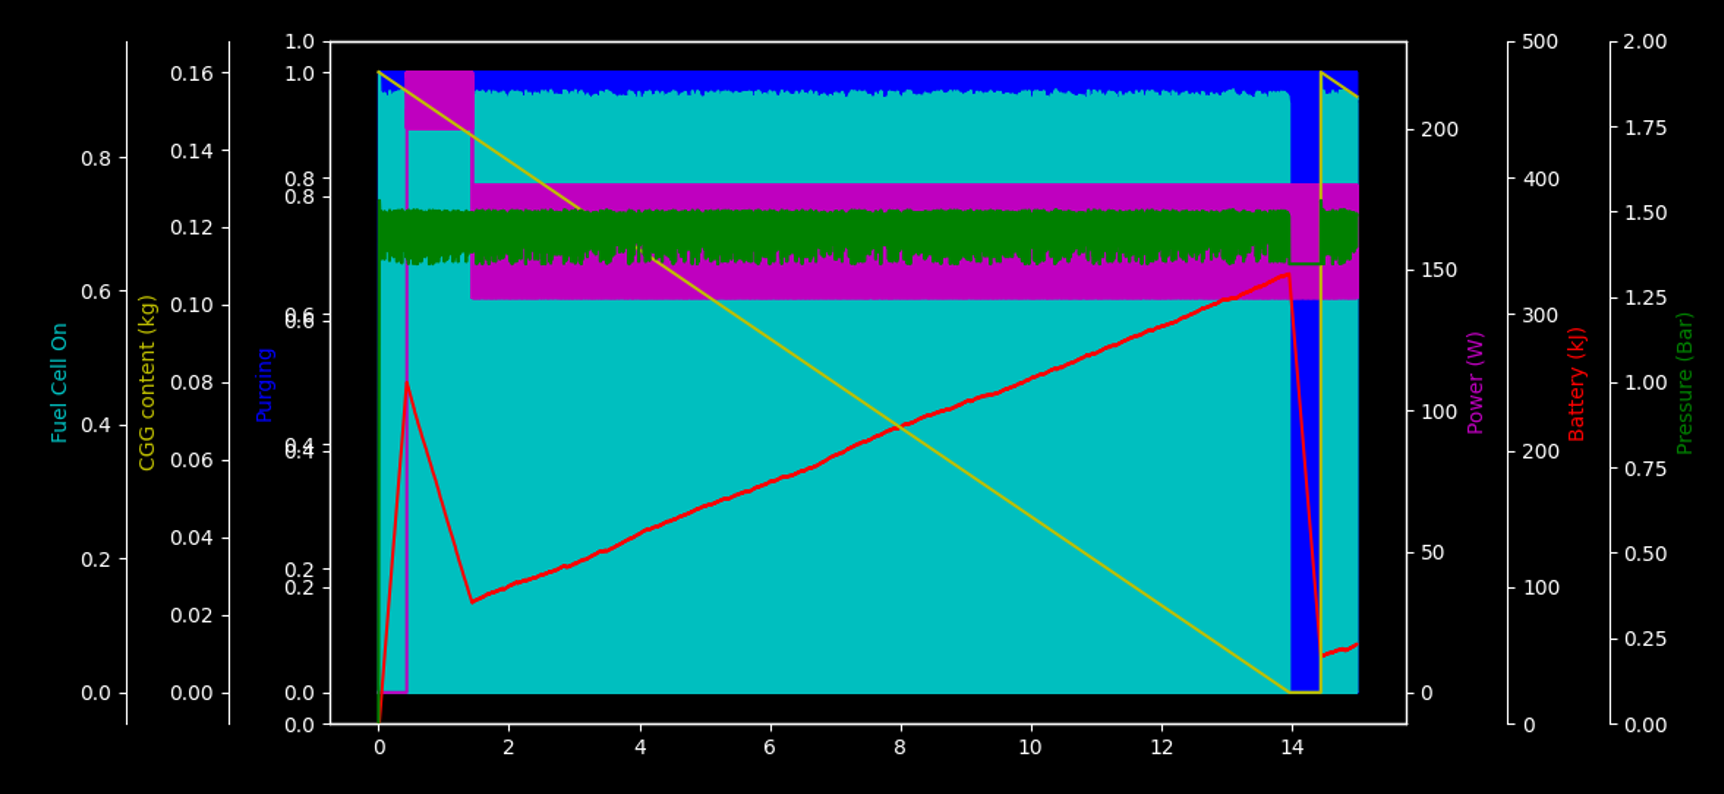
\includegraphics[width=\textwidth]{media/sim/default.png}
    \caption{Simulation Result}
    \label{fig:sim default}
\end{figure}

The green, blue and cyan lines indicate pressure in the buffer volume, whether a purge event is happening and how much power the fuel cell produces respectively. At the scale of figure~\ref{fig:sim default} their behaviour is poorly visible. Figure~\ref{fig:sim purge} provides a zoomed in view around the moment that a purge event is happening, there the behaviour of the three lines is better visible. Note however, that some lines have been excluded from this view and the scales have been altered for better visibility.

The blue line is at zero when no purge event is happening and jumps to one during a purge event. In the middle of the graph a purge event of around two seconds is visible. During the purge event the fuel cell uses hydrogen at an increased rate. Consequently, the pressure in the buffer volume drops to supply this extra hydrogen which can be seen in the green line. The controller notices this pressure drop and limits the power output of the fuel cell thereby limiting the hydrogen consumption, this can be seen by the cyan line dropping to zero.

After the purge event, the fuel cell is still limited, allowing the pressure in the buffer volume to build up again. When this pressure has been largely recovered, the fuel cell is allowed to produce power again. The reduction in power output from the fuel cell is compensated by the battery, which is visible in the red line.

\begin{figure}[htp]
    \centering
    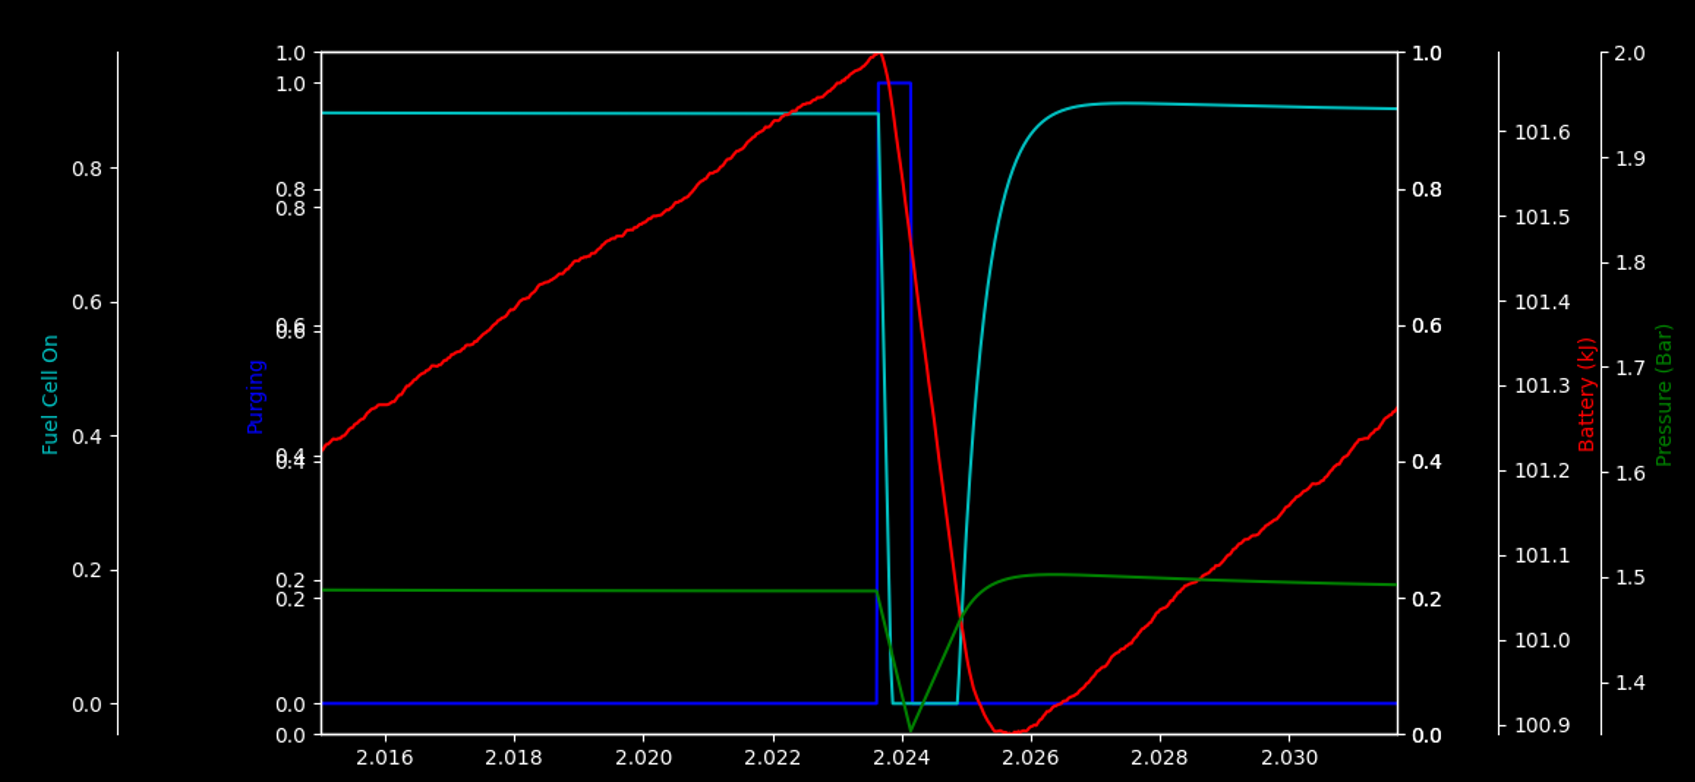
\includegraphics[width=\textwidth]{media/sim/purge.png}
    \caption{Purge Event}
    \label{fig:sim purge}
\end{figure}

\newpage
Many of the parameters used in this simulation were altered to investigate their effect on the overall system behaviour. These results were used during the design of the hydrogen power system, and as such will be discussed further in chapter~\ref{chap:design}.

The simulation results will also need to be verified against real-world test results. For this and other purposes a compressed air system will be developed that will perform the gas flow of the hydrogen power system but with compressed air instead of hydrogen. This air-equivalent system will be discussed throughout the following chapters. Its results will be compared with the results of this simulation in chapter~\ref{chap:testing}.


\section{Air Equivalent Test Setup}%
\label{sec:air design}
TBD


\subsection{Fuel Supply Regulator}
TBD

\begin{figure}[htp]
    \begin{subfigure}{0.5\textwidth}%
        \centering%
        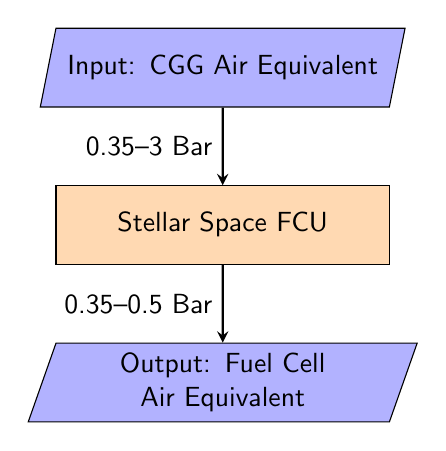
\begin{tikzpicture}[node distance=2 cm]
            \node (in) [io] {Input: CGG Air Equivalent};
            \node (valve) [process, below of=in] {Stellar Space FCU};
            \node (out) [io, below of=valve] {Output: Fuel Cell Air Equivalent};

            \draw [arrow] (in) -- node[anchor=east] {0.35--3 Bar} (valve);
            \draw [arrow] (valve) -- node[anchor=east] {0.35--0.5 Bar} (out);
        \end{tikzpicture}%
        \caption{FCU}%
        \label{fc:fcu}%
    \end{subfigure}%
    \hfill%
    \begin{subfigure}{0.5\textwidth}%
        \centering%
        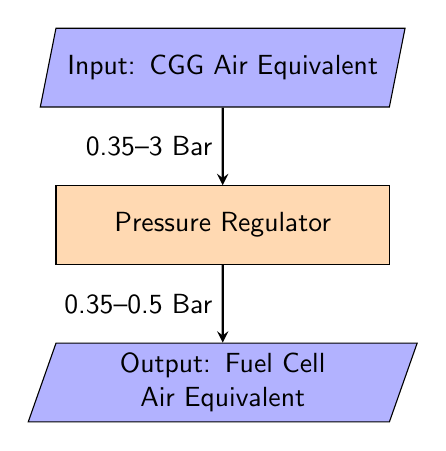
\begin{tikzpicture}[node distance=2 cm]
            \node (in) [io] {Input: CGG Air Equivalent};
            \node (valve) [process, below of=in] {Pressure Regulator};
            \node (out) [io, below of=valve] {Output: Fuel Cell Air Equivalent};

            \draw [arrow] (in) -- node[anchor=east] {0.35--3 Bar} (valve);
            \draw [arrow] (valve) -- node[anchor=east] {0.35--0.5 Bar} (out);
        \end{tikzpicture}%
        \caption{Pressure Regulator}%
        \label{fc:regulator}%
    \end{subfigure}%

    \caption{Compressed Air Equivalent}%
    \label{fc:air equivalent}%
\end{figure}%
\clearpage


\subsection{Cool Gas Generator}
TBD
\begin{figure}[htp]
    \begin{subfigure}{0.5\textwidth}%
        \centering%
        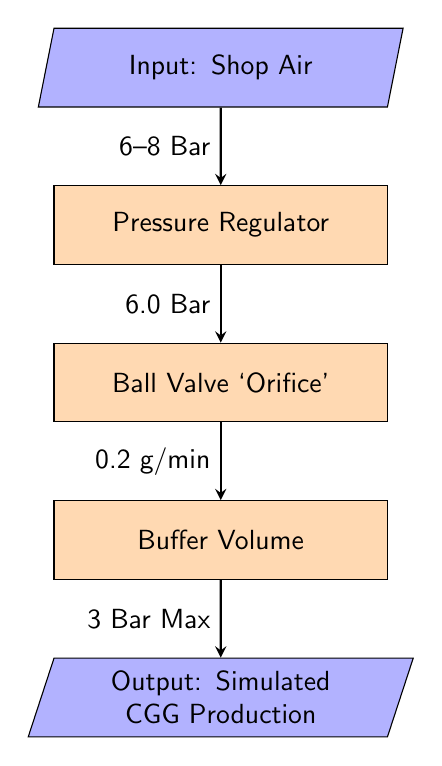
\begin{tikzpicture}[node distance=2 cm]
            \node (in1) [io] {Input: Shop Air};
            \node (pro1) [process, below of=in1] {Pressure Regulator};
            \node (pro2) [process, below of=pro1] {Ball Valve `Orifice'};
            \node (pro3) [process, below of=pro2] {Buffer Volume};
            \node (out1) [io, below of=pro3] {Output: Simulated CGG Production};

            \draw [arrow] (in1) -- node[anchor=east] {6--8 Bar} (pro1);
            \draw [arrow] (pro1) -- node[anchor=east] {6.0 Bar} (pro2);
            \draw [arrow] (pro2) -- node[anchor=east] {0.2 g/min} (pro3);
            \draw [arrow] (pro3) -- node[anchor=east] {3 Bar Max} (out1);
        \end{tikzpicture}%
        \caption{Ball Valve}%
        \label{fc:ball cgg}%
    \end{subfigure}%
    \hfill%
    \begin{subfigure}{0.5\textwidth}%
        \centering%
        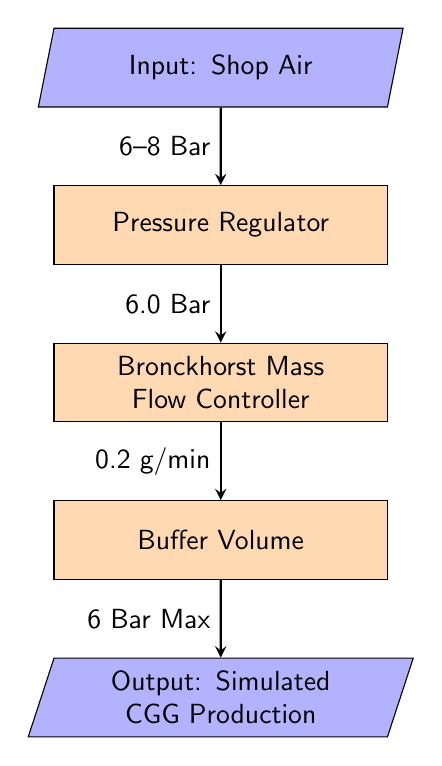
\begin{tikzpicture}[node distance=2 cm]
            \node (in1) [io] {Input: Shop Air};
            \node (pro1) [process, below of=in1] {Pressure Regulator};
            \node (pro2) [process, below of=pro1] {Bronckhorst Mass Flow Controller};
            \node (pro3) [process, below of=pro2] {Buffer Volume};
            \node (out1) [io, below of=pro3] {Output: Simulated CGG Production};

            \draw [arrow] (in1) -- node[anchor=east] {6--8 Bar} (pro1);
            \draw [arrow] (pro1) -- node[anchor=east] {6.0 Bar} (pro2);
            \draw [arrow] (pro2) -- node[anchor=east] {0.2 g/min} (pro3);
            \draw [arrow] (pro3) -- node[anchor=east] {6 Bar Max} (out1);
        \end{tikzpicture}%
        \caption{Bronckhorst}%
        \label{fc:bronckhorst cgg}%
    \end{subfigure}%

    \caption{CGG Compressed Air Equivalent}%
    \label{fc:cgg equivalent}%
\end{figure}%
\clearpage


\subsection{Fuel Cell}
TBD
\begin{figure}[htp]
    % \centering%
    \begin{subfigure}{\textwidth}%
        \centering%
        \scalebox{0.9}{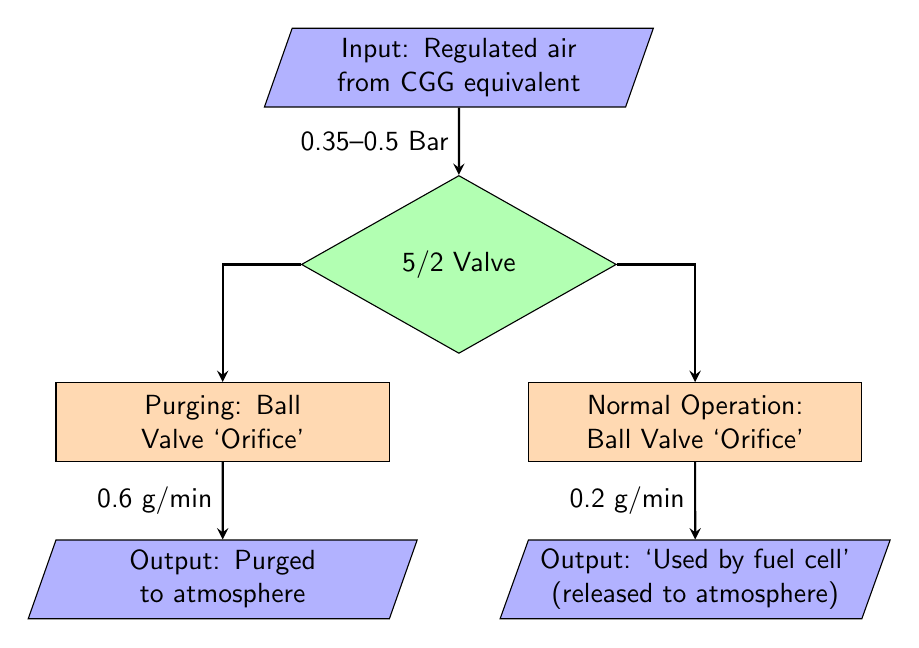
\begin{tikzpicture}[node distance=2 cm]
                \node (in) [io] {Input: Regulated air from CGG equivalent};
                \node (valve) [decision, below of=in, yshift=-5mm] {5/2 Valve};
                \node (purge) [process, below of=valve, xshift = -3cm] {Purging: Ball Valve `Orifice'};
                \node (normal) [process, below of=valve, xshift = 3cm] {Normal Operation: Ball Valve `Orifice'};
                \node (outp) [io, below of=purge] {Output: Purged to atmosphere};
                \node (outn) [io, below of=normal] {Output: `Used by fuel cell' (released to atmosphere)};

                \draw [arrow] (in) -- node[anchor=east] {0.35--0.5 Bar} (valve);
                \draw [arrow] (valve) -| (purge);
                \draw [arrow] (valve) -| (normal);
                \draw [arrow] (purge) -- node[anchor=east] {0.6 g/min} (outp);
                \draw [arrow] (normal) -- node[anchor=east] {0.2 g/min} (outn);
            \end{tikzpicture}}%
        \caption{Ball Valve, Single Switch}%
        \label{fc:ball fc}%
    \end{subfigure}%

    \vspace{1cm}
    \begin{subfigure}{\textwidth}%
        \centering%
        \scalebox{0.9}{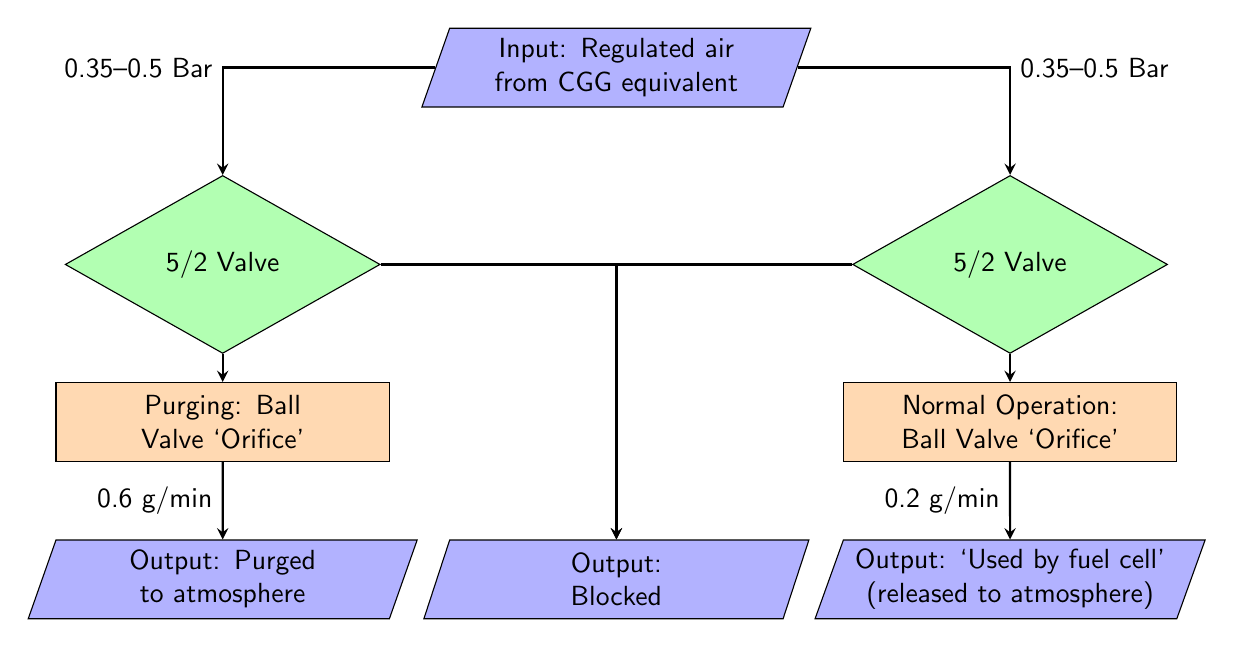
\begin{tikzpicture}[node distance=2 cm]
                \node (in) [io] {Input: Regulated air from CGG equivalent};
                \node (pvalve) [decision, below of=in, yshift=-5mm, xshift=-5cm] {5/2 Valve};
                \node (nvalve) [decision, below of=in, yshift=-5mm, xshift=5cm] {5/2 Valve};
                \node (porifice) [process, below of=pvalve] {Purging: Ball Valve `Orifice'};
                \node (norifice) [process, below of=nvalve] {Normal Operation: Ball Valve `Orifice'};
                \node (pout) [io, below of=porifice] {Output: Purged to atmosphere};
                \node (nout) [io, below of=norifice] {Output: `Used by fuel cell' (released to atmosphere)};
                \node (block) [io, below of= in, yshift=-4.5cm] {Output:\\Blocked};


                \draw [arrow] (in) -| node[anchor=east] {0.35--0.5 Bar} (pvalve);
                \draw [arrow] (in) -| node[anchor=west] {0.35--0.5 Bar} (nvalve);
                \draw [arrow] (pvalve) -- (porifice);
                \draw [arrow] (nvalve) -- (norifice);
                \draw [arrow] (pvalve) -| (block);
                \draw [arrow] (nvalve) -|    (block);
                \draw [arrow] (porifice) -- node[anchor=east] {0.6 g/min} (pout);
                \draw [arrow] (norifice) -- node[anchor=east] {0.2 g/min} (nout);
            \end{tikzpicture}}%
        \caption{Ball Valve, Dual Switch}%
        \label{fc:ball fc}%
    \end{subfigure}%

    \vspace{1cm}
    \begin{subfigure}{\textwidth}%
        \centering%
        \scalebox{0.9}{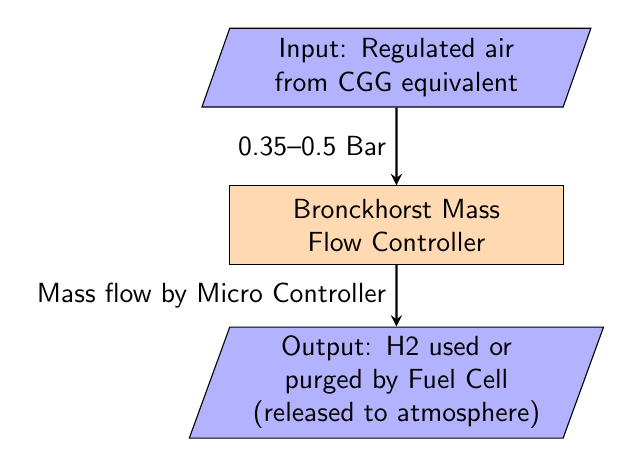
\begin{tikzpicture}[node distance=2 cm]
                \node (in) [io] {Input: Regulated air from CGG equivalent};
                \node (valve) [process, below of=in] {Bronckhorst Mass Flow Controller};
                \node (out) [io, below of=valve] {Output: H2 used or purged by Fuel Cell (released to atmosphere)};

                \draw [arrow] (in) -- node[anchor=east] {0.35--0.5 Bar} (valve);
                \draw [arrow] (valve) -- node[anchor=east] {Mass flow by Micro Controller} (out);
            \end{tikzpicture}}%
        \caption{Bronckhorst}%
        \label{fc:bronckhorst fc}%
    \end{subfigure}%

    \caption{Fuel Cell Compressed Air Equivalent}%
    \label{fc:fc equivalent}%
\end{figure}%

\begin{tabularx}{\textwidth}{lXX}
    \toprule
    \textbf{Test setup}      & \textbf{Capabilities}              & \textbf{Downsides}                                         \\
    \midrule
    Ball Valve Single Switch & Test uncontrolled system behaviour & Mass flow is only accurate when input pressure is constant \\
    Ball Valve Dual Switch   & Test On--Off controlled behaviour  & Mass flow is only accurate when input pressure is constant \\
    Bronchorst Valve         & Test PID controlled behaviour      & Expensive                                                  \\
    \bottomrule
\end{tabularx}
\newpage


\section{Hydrogen Test Setup}


\begin{table}[htp]
    \begin{tabularx}{\textwidth}{lXXX}
        \toprule
        \textbf{Name}                                                                                                                                                          & \textbf{H-100}                                      & \textbf{H-200} & \textbf{H2Gatech} \\
        \midrule
        \textbf{Image}                                                                                                                                                         &
        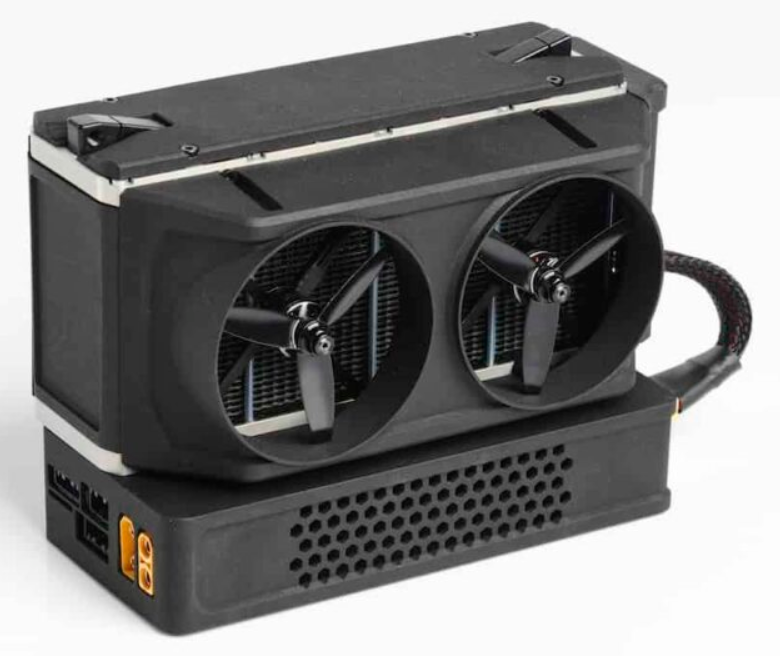
\includegraphics[width=\linewidth]{media/fc1.png}                                                                                                                      &
        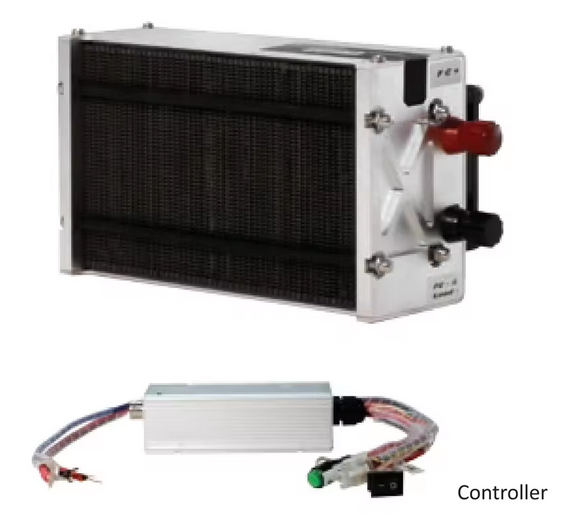
\includegraphics[width=\linewidth]{media/fc2.png}                                                                                                                      &
        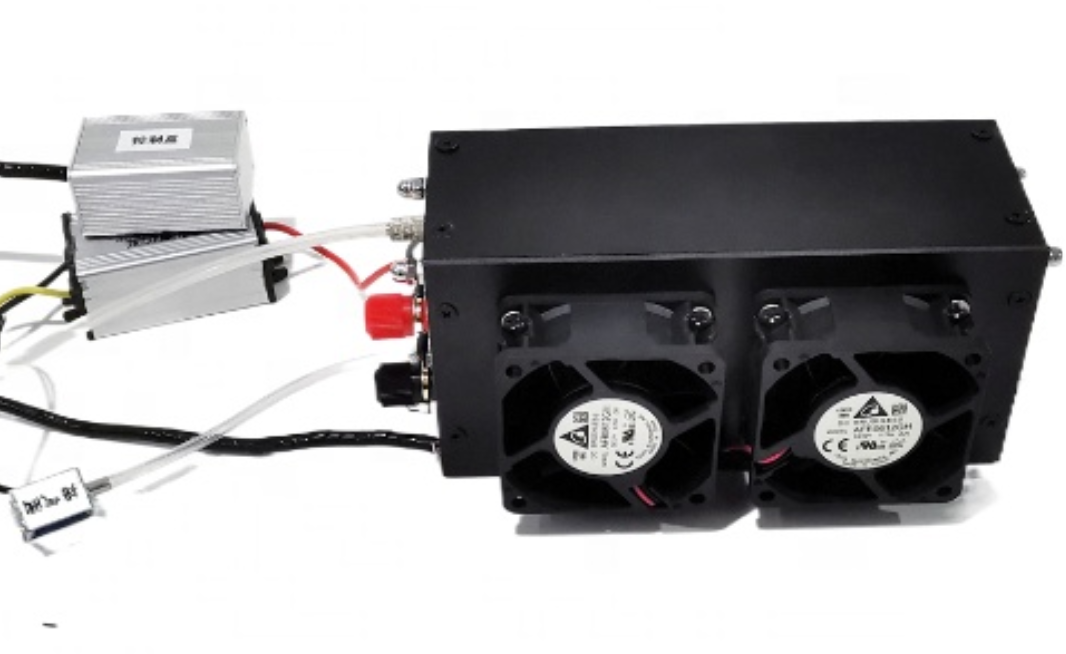
\includegraphics[width=\linewidth]{media/fc3.png}                                                                                                                                                                                                                 \\
        \midrule
        \textbf{Power}                                                                                                                                                         & 100 W                                               & 200 W          & 100 W             \\
        \textbf{Price}                                                                                                                                                         & € 775                                               & € 1164         & € 715             \\
        \textbf{Link}                                                                                                                                                          &
        {\href{https://www.alibaba.com/product-detail/100W-Integrated-PEM-Hydrogen-Fuel-Cell_1601282328019.html?spm=a2700.galleryofferlist.normal_offer.d_title.792d13a09NNM3m & priceId=0d1b025c670b42c8945b940e159741ea}{alibaba}} &
        {\href{https://www.alibaba.com/product-detail/200W-Hydrogen-Fuel-Cell-Ideal-for_1601282060741.html}{alibaba}}                                                          &
        {\href{https://www.alibaba.com/product-detail/Long-Life-Cycle-PEM-Hydrogen-Fuel_1601624915790.html?spm=a2700.galleryofferlist.normal_offer.d_title.792d13a09NNM3m      & priceId=0d1b025c670b42c8945b940e159741ea}{alibaba}}                                      \\
        \textbf{Shipping}                                                                                                                                                      & $\pm$1 month                                        & $\pm$1 month   & 5--20 Days        \\
        \bottomrule
    \end{tabularx}
\end{table}

\clearpage



\chapter{Test Results}%
\label{chap:testing}
\emph{This chapter presents the test methodology and results of the python simulation, compressed air equivalent and hydrogen test bench. The simulation shows expected behaviour of hydrogen pressure during purge events, which is then validated using the results of the compressed air equivalent test. The similarity between the results of these tests show great promise for the hydrogen test bench which is yet to be tested.}

\todo{Rewrite when hydrogen tests are complete}

\newpage




% Goals of various tests:
% \begin{itemize}
%     \item Compressed Air Equivalent Test
%           \begin{itemize}
%               \item Explore unknown risks
%               \item Verify expected system behaviour
%               \item Verify simulation results
%               \item Compare control strategies
%           \end{itemize}

%     \item FCU Pressure test
%           \begin{itemize}
%               \item Verify consistency of FCU output pressure
%           \end{itemize}

%     \item FCU mass flow test
%           \begin{itemize}
%               \item Verify consistency of FCU output mass flow
%               \item Verify leakage of FCU
%           \end{itemize}

%     \item Gas supply test
%           \begin{itemize}
%               \item Verify consistency of gas pressure during purge events
%               \item Verify consistency of gas mass flow during purge events
%               \item Verify total leakage of gas supply system
%           \end{itemize}

%     \item Fuel Cell test
%           \begin{itemize}
%               \item Verify the fuel cell is working normally
%               \item Verify the fuel cell output voltage
%               \item Verify the fuel cell output power
%               \item Verify the fuel cell fuel consumption
%           \end{itemize}

%     \item Propulsion test
%           \begin{itemize}
%               \item Verify the maximum thrust
%               \item Verify the maximum power draw
%               \item Verify the relation between input power and thrust output
%           \end{itemize}

%     \item Hybrid Battery test
%           \begin{itemize}
%               \item Verify the battery cannot back-feed power into the fuel cell
%               \item Verify output power of hybrid system
%               \item Verify output voltage of hybrid system
%           \end{itemize}

%     \item Integration test
%           \begin{itemize}
%               \item Verify all individually tested components behave as expected when integrated into one system
%               \item Verify relation between fuel consumption and thrust output
%           \end{itemize}
% \end{itemize}

% \clearpage

\section{Python Simulation}

Running the simulation in its base form, with all parameters unchanged and as stated in table~\ref{tab:sim_parameters} produces the graph in figure~\ref{fig:sim default}. The pink line represents the power draw from the drone, this illustrates most clearly what phase of the mission is currently happening. Takeoff happens around half an hour into the simulation, then a 1 hour climb with high power demand after which the drone cruises for the rest of the mission, using less power. As a range was given for both climb and cruise power the simulation picks a random value in the range each timestep, hence this line appears very thick.

The red line represents the content of the battery. It starts empty and begins to charge, when it is at 50\% the drone starts liftoff. This uses more power than the fuel cell can provide, therefore the battery supplies the additional power and thus discharges over time. When the drone switches to cruising the battery can charge again slowly. Note how the battery discharges rapidly around the 14 hour mark. This is because the CGG has run out (indicated by the yellow line) and the fuel cell can no longer provide any power. At this point, all the power is delivered by the battery until it is at 10\%, then the mission is at an end or a new CGG is ignited in case multiple CGG's were brought on the mission.

\begin{figure}[htp]
    \centering
    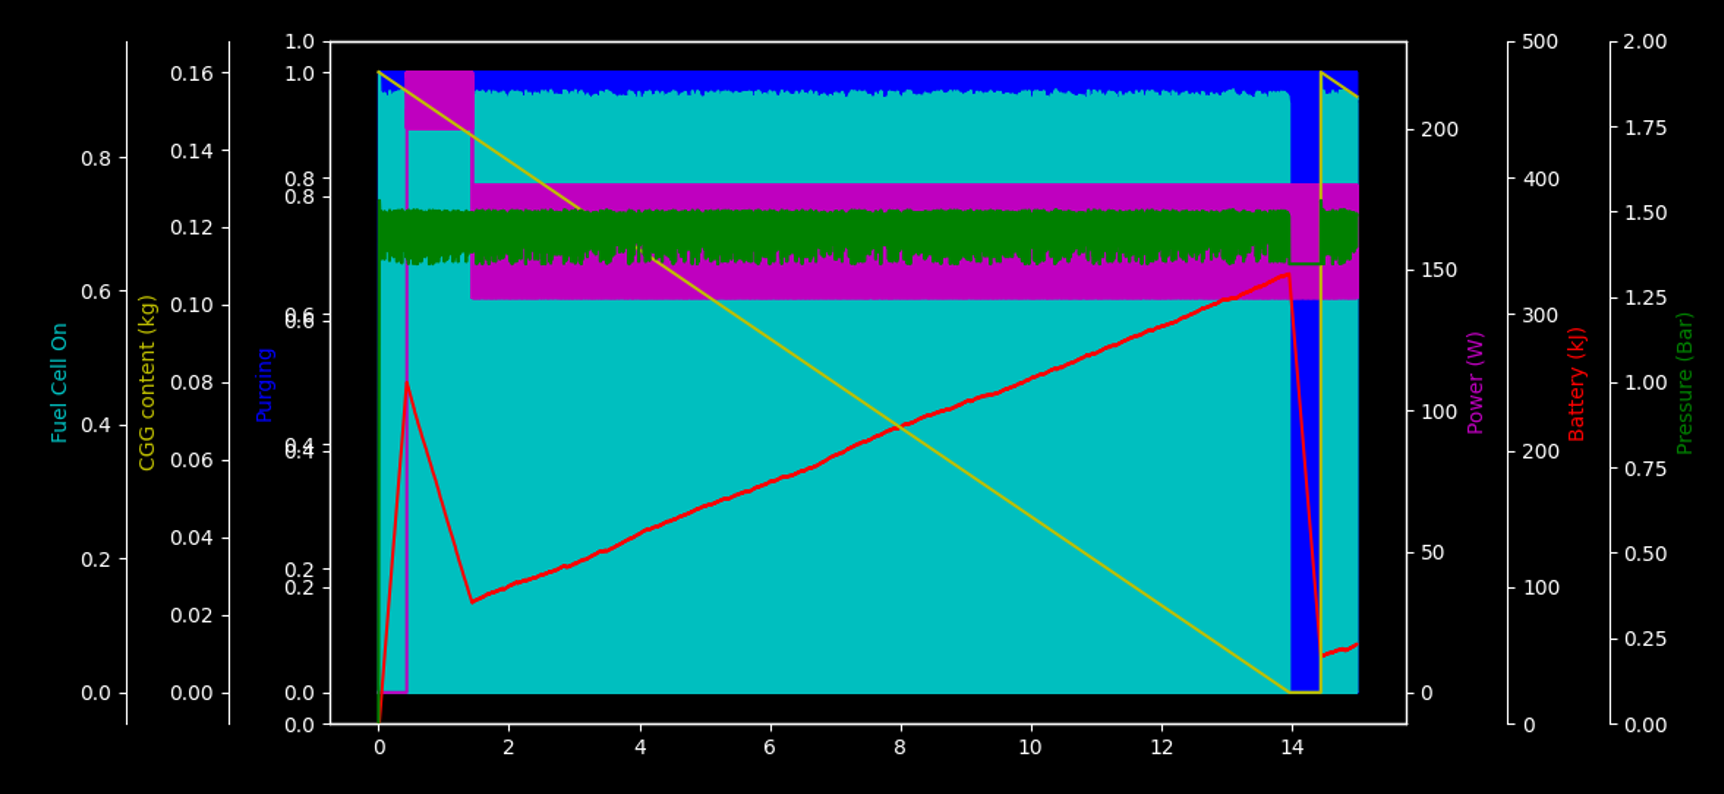
\includegraphics[width=\textwidth]{media/sim/default.png}
    \caption{Simulation Result}
    \label{fig:sim default}
\end{figure}

The green, blue and cyan lines indicate pressure in the buffer volume, whether a purge event is happening and how much power the fuel cell produces respectively. At the scale of figure~\ref{fig:sim default} their behaviour is poorly visible. Figure~\ref{fig:sim purge} provides a zoomed in view around the moment that a purge event is happening, there the behaviour of the three lines is better visible. Note however, that some lines have been excluded from this view and the scales have been altered for better visibility.

The blue line is at zero when no purge event is happening and jumps to one during a purge event. In the middle of the graph a purge event of around two seconds is visible. During the purge event the fuel cell uses hydrogen at an increased rate. Consequently, the pressure in the buffer volume drops to supply this extra hydrogen which can be seen in the green line. The controller notices this pressure drop and limits the power output of the fuel cell thereby limiting the hydrogen consumption, this can be seen by the cyan line dropping to zero.

After the purge event, the fuel cell is still limited, allowing the pressure in the buffer volume to build up again. When this pressure has been largely recovered, the fuel cell is allowed to produce power again. The reduction in power output from the fuel cell is compensated by the battery, which is visible in the red line.

\begin{figure}[htp]
    \centering
    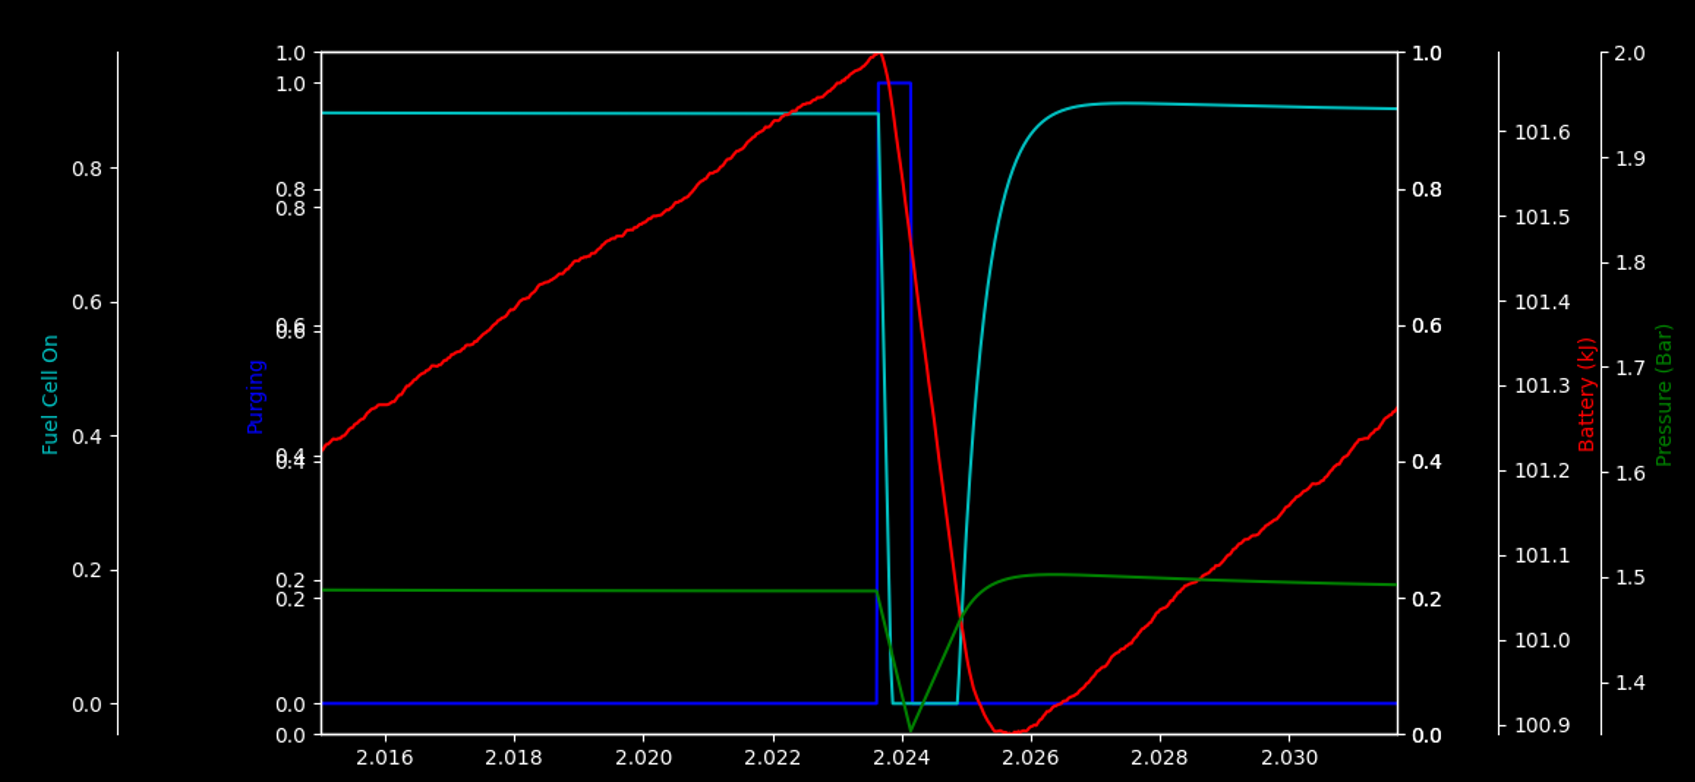
\includegraphics[width=\textwidth]{media/sim/purge.png}
    \caption{Purge Event}
    \label{fig:sim purge}
\end{figure}

\newpage
% Many of the parameters used in this simulation were altered to investigate their effect on the overall system behaviour. These results were used during the design of the hydrogen power system, and as such will be discussed further in chapter~\ref{sec:air design}.

The simulation results will also need to be verified against real-world test results. For this and other purposes the compressed air equivalent system was developed that will perform the gas flow of the hydrogen power system but with compressed air instead of hydrogen. Section~\ref{sec:air results} will compare the results from the simulation with the compressed air equivalent system.

% \todo{Results with different parameters}
The simulation can also be run with different parameters. Figure~\ref{fig:1cgg low} and~\ref{fig:1cgg high} show the simulation results with the average cruise power set to the lower and upper bound respectively. There can be seen that when the power consumption is high, the fuel cell is just capable of charging the battery. When the power consumption is low however, the battery must charge faster to absorb the excess electricity, which results in it being fully charged after about five hours. Excess hydrogen then builds pressure in the buffer volume quickly and eventually escapes through the pressure relief valve. 18.5 grams of hydrogen was vented and thus not used to generate power.

Figure~\ref{fig:4cgg low} shows the same lower limit but with four CGG's containing a quarter of the hydrogen each. This allows the battery to discharge after a CGG runs out, preventing this wasted hydrogen. Consequently the flight with four CGGs lasted over 15 hours, compared to less than 14 with only one CGG.

Cruise power and CGG amount are only two of the many configurable parameters listed in table~\ref{tab:sim_parameters}. The configurability of this simulation allows it to also be used in architecture design choices for the larger SHARP project.
\begin{figure}[htp]
    \begin{subfigure}{\textwidth}
        \centering
        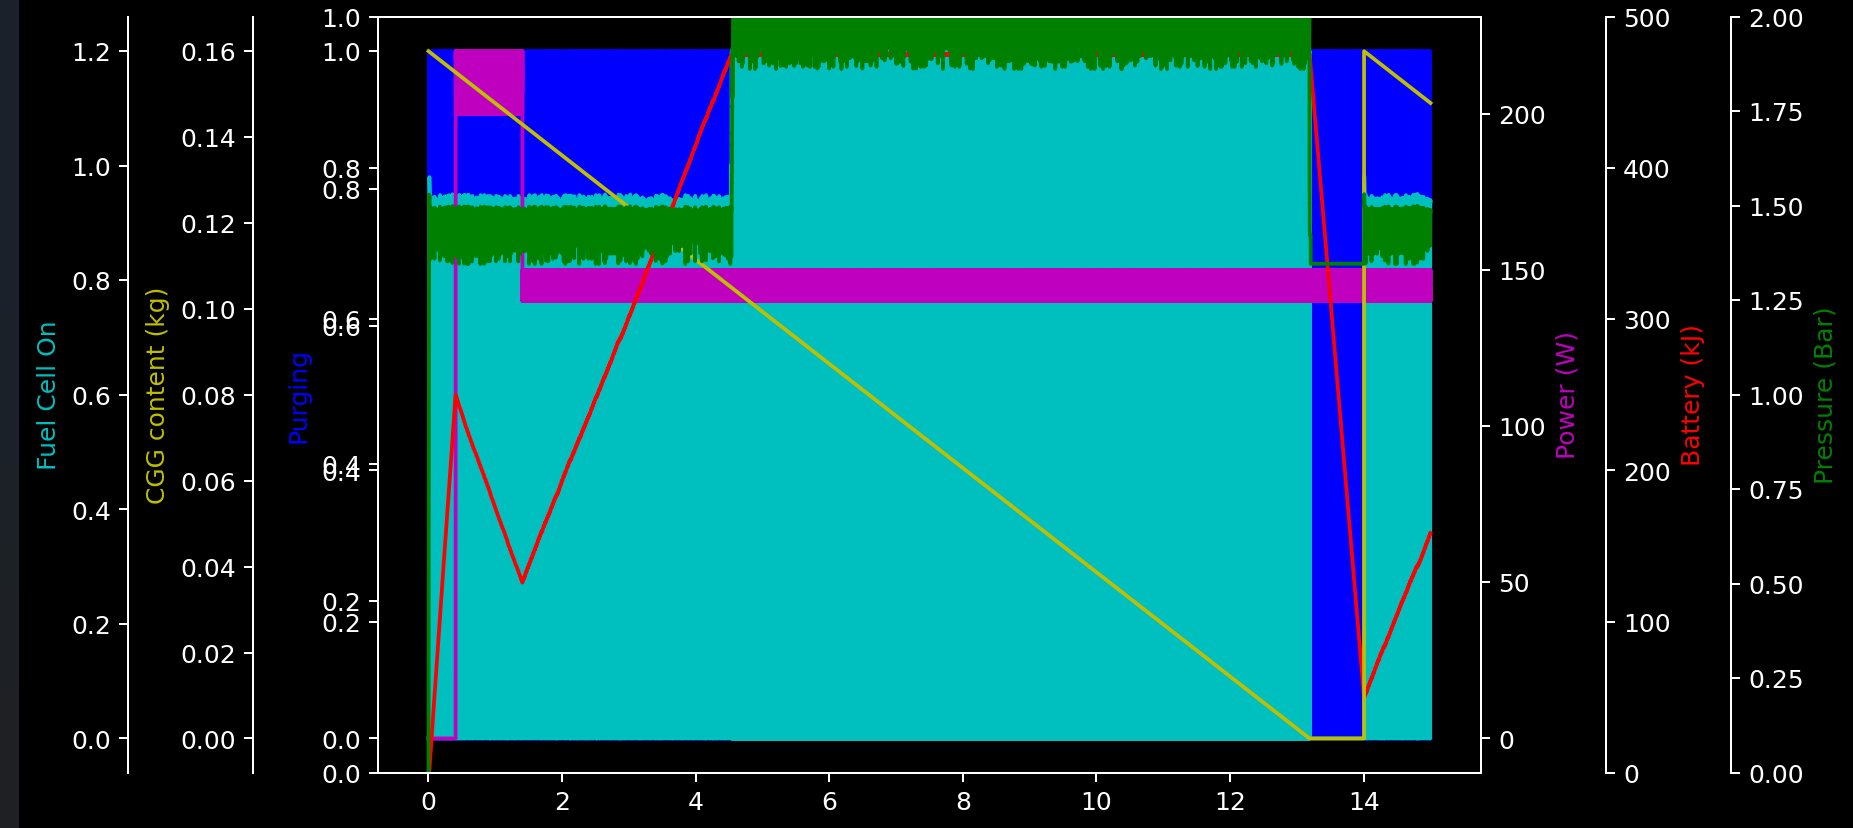
\includegraphics[width=\textwidth]{media/sim/1cgg low.png}
        \caption{Simulation with 1 CGG and 145 W cruise power}
        \label{fig:1cgg low}
    \end{subfigure}
    \begin{subfigure}{\textwidth}
        \centering
        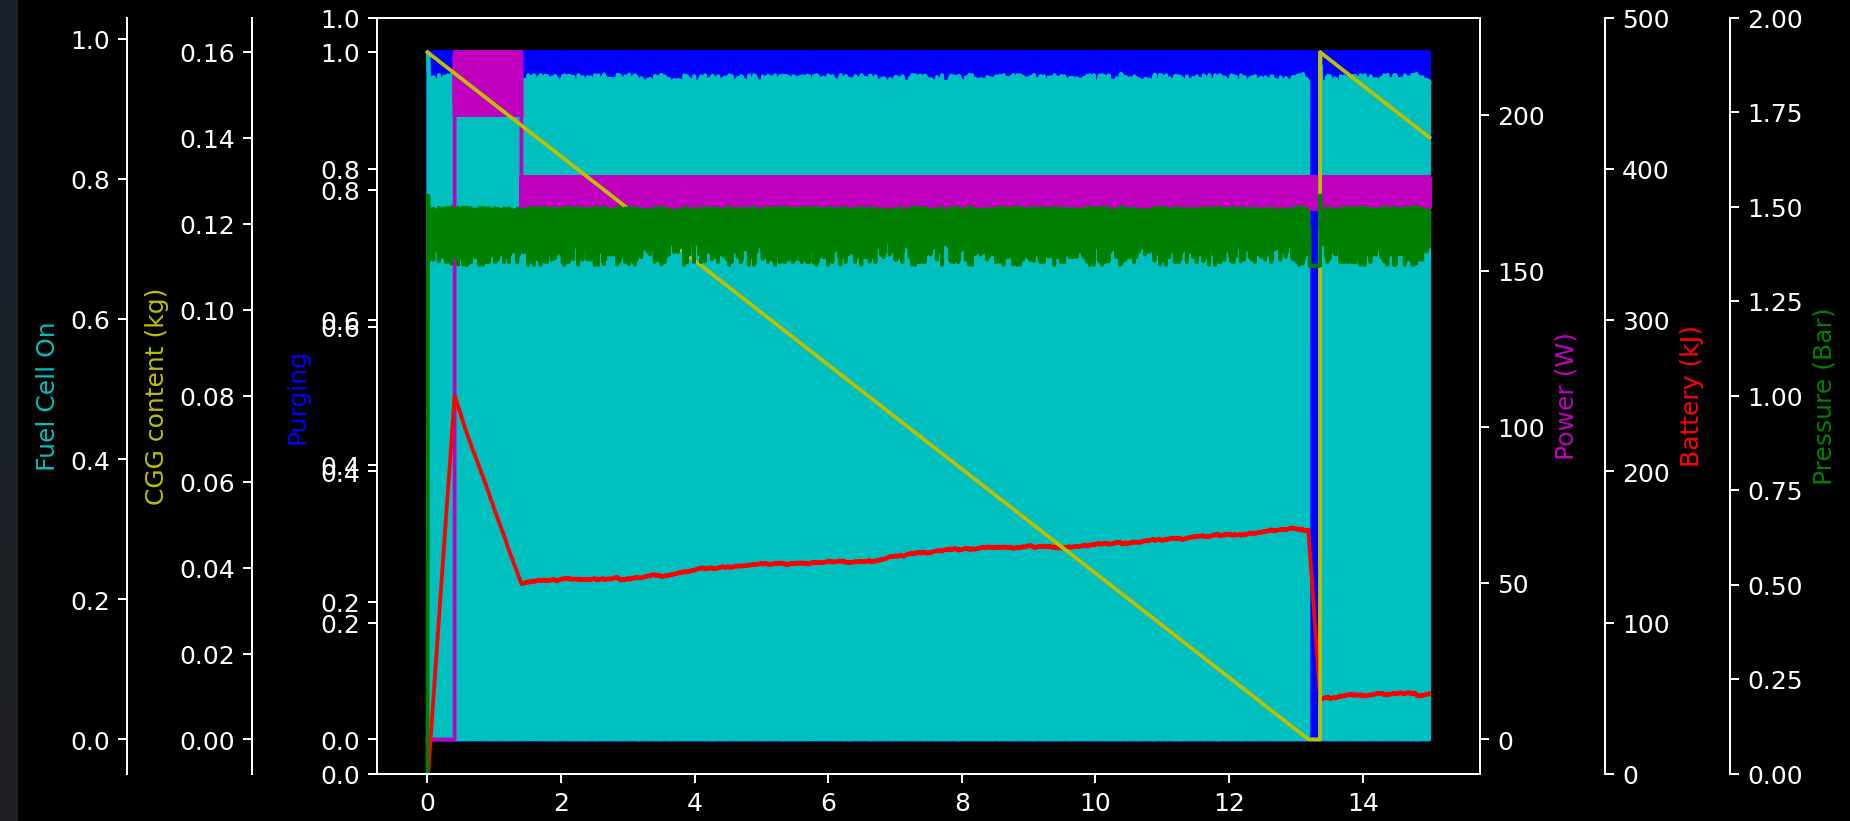
\includegraphics[width=\textwidth]{media/sim/1cgg high.png}
        \caption{Simulation with 1 CGG and 175 W cruise power}
        \label{fig:1cgg high}
    \end{subfigure}
    \begin{subfigure}{\textwidth}
        \centering
        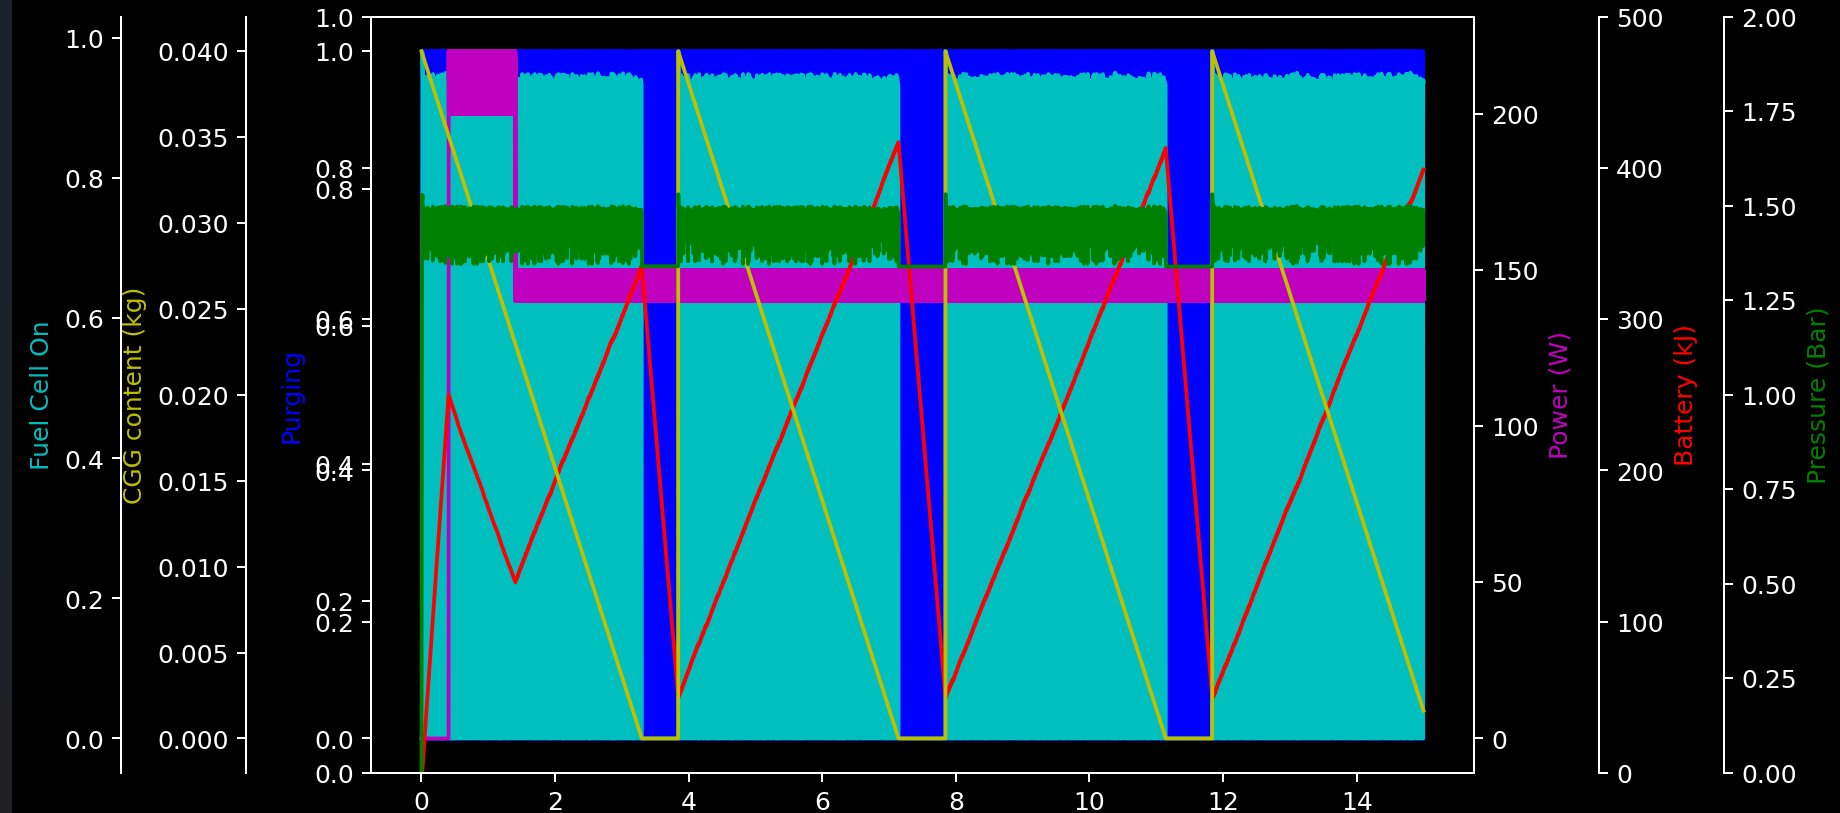
\includegraphics[width=\textwidth]{media/sim/4cgg low.png}
        \caption{Simulation with 4 CGG and 145 W cruise power}
        \label{fig:4cgg low}
    \end{subfigure}
    \caption{Simulation with different parameters}
    \label{fig:sim parameter results}
\end{figure}

% \begin{figure}[htp]
%     \centering
%     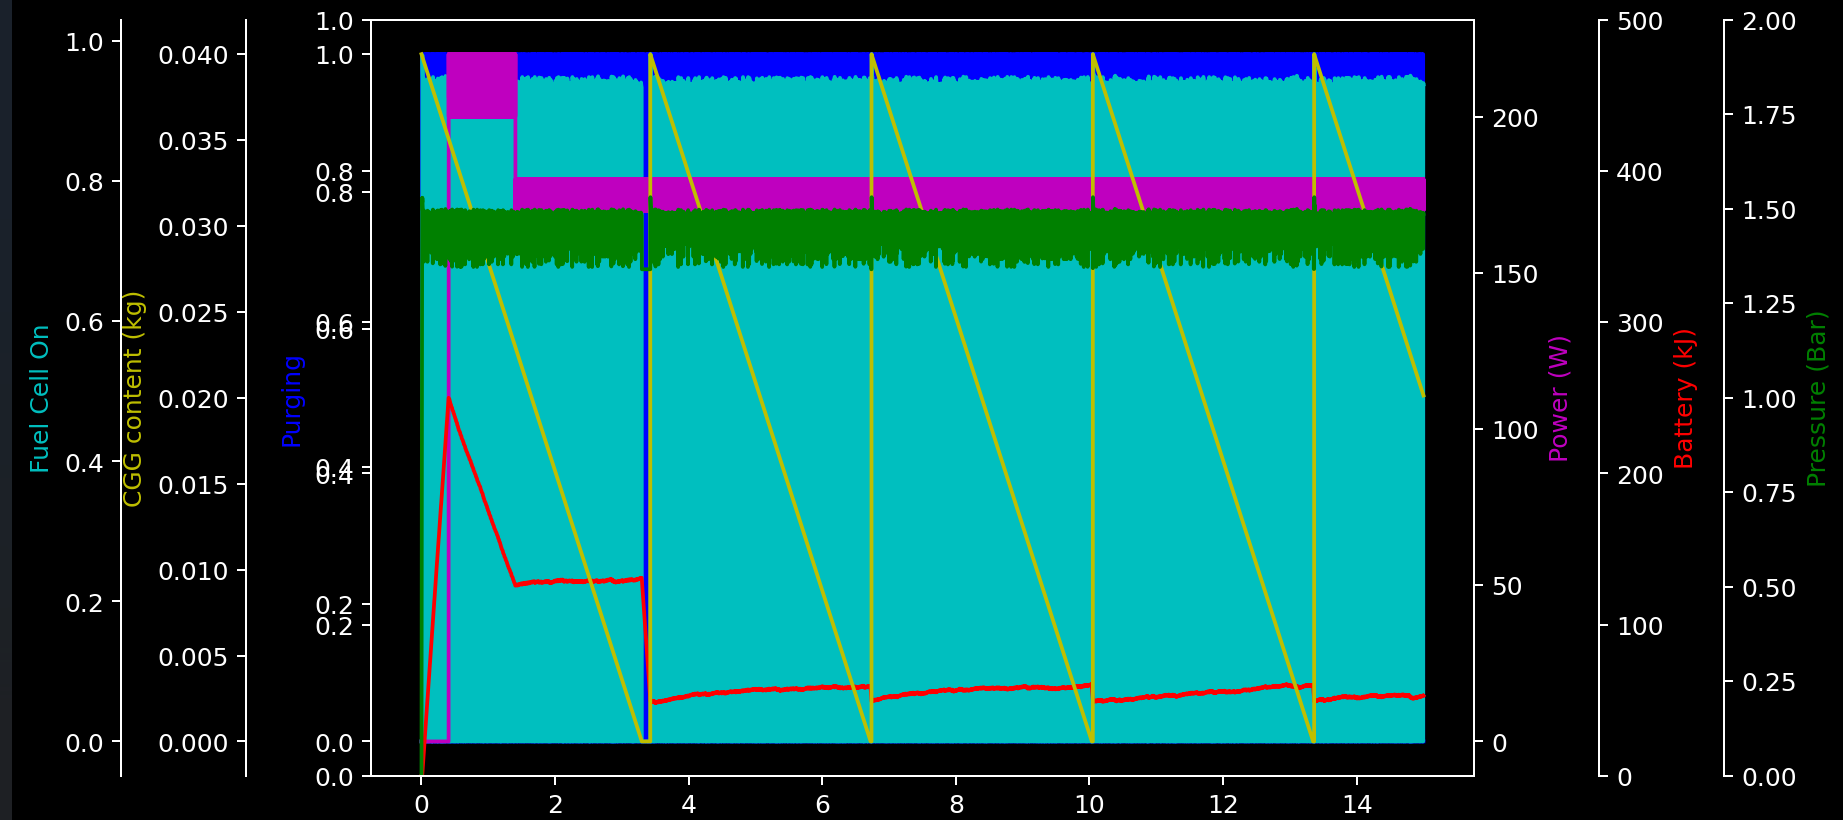
\includegraphics[width=\textwidth]{media/sim/4cgg high.png}
%     \caption{Simulation with 4 CGG and 175 W cruise power}
%     \label{fig:4cgg high}
% \end{figure}
\newpage
%

\section{Compressed Air Equivalent}

\emph{The compressed air equivalent system performs the same gas flows as the hydrogen part of the power generation and feed system. This system will allow analysis of the flow dynamics of the system without the use of hydrogen, allowing for a cheaper and safer system that is faster to realise. In this chapter, an overview is given of the system and the tests performed with it. The results of these tests are reviewed and compared with those of the python simulation.}

\subsection*{Testing Goals}
The main goal of the compressed air equivalent tests is to explore the flow dynamics of the system and verify that they match expected behaviour. This includes comparing results with the python simulation and verifying that using the internal volume of the CGG as a buffer is sufficient to ensure stable flow to the fuel cell during purge events.

Additionally, the compressed air tests will be used to gain experience with the fluidics hardware and explore risks like leakage before introducing hydrogen.


% Goals of compressed air equivalent tests:
% \begin{itemize}
%     \item Explore unknown risks
%     \item Verify expected system behaviour
%     \item Verify simulation results
%     \item Compare control strategies
% \end{itemize}


\subsection*{Results}
Figure~\ref{fig:air purge} show the pressure in the CGG buffer volume and the flow rate from the CGG to the fuel cell. Figure~\ref{fig:sim purge} shows the results of the python simulation during a similar time frame. The simulation also shows the pressure in the CGG buffer volume in green, which can be directly compared to the measure pressure in the air test. The simulation does not directly show the same flow rate. However, it does show the state of the fuel cell from which a flow rate can be inferred. The blue line in the simulation shows when the fuel cell is in purge mode, which corresponds to the higher flow rate in the air test. The cyan line shows when the fuel cell is in normal mode, which corresponds to the lower flow rate in the air test.

\emph{Note that the graph representing the flow rate of the air system has been scaled to improve visibility, this means that its units are no longer correct.}

During normal operation, the fuel cell consumes slightly more than the CGG produces, which causes the pressure in the buffer to decrease. When the pressure drops too low, the fuel cell is temporarily disabled to allow the buffer to fill up again. This behaviour is seen in both the simulation and the test results. The real system reacts a bit slower to the pressure changes than the simulation, which leads to slightly larger pressure fluctuations. However, the overall behaviour is very similar, which gives confidence that the simulation is accurately capturing the flow dynamics of the system.

When a purge event occurs, the fuel cell equivalent briefly consumes a lot more air, which causes a sharp drop in pressure. This too occurs both in the simulation and in the test results. In both systems the pressure drops from around 3.4 Bar to around 2 Bar. After the purge event, both systems disable the fuel cell to fill up the buffer again.

\begin{figure}
    \begin{subfigure}{\textwidth}
        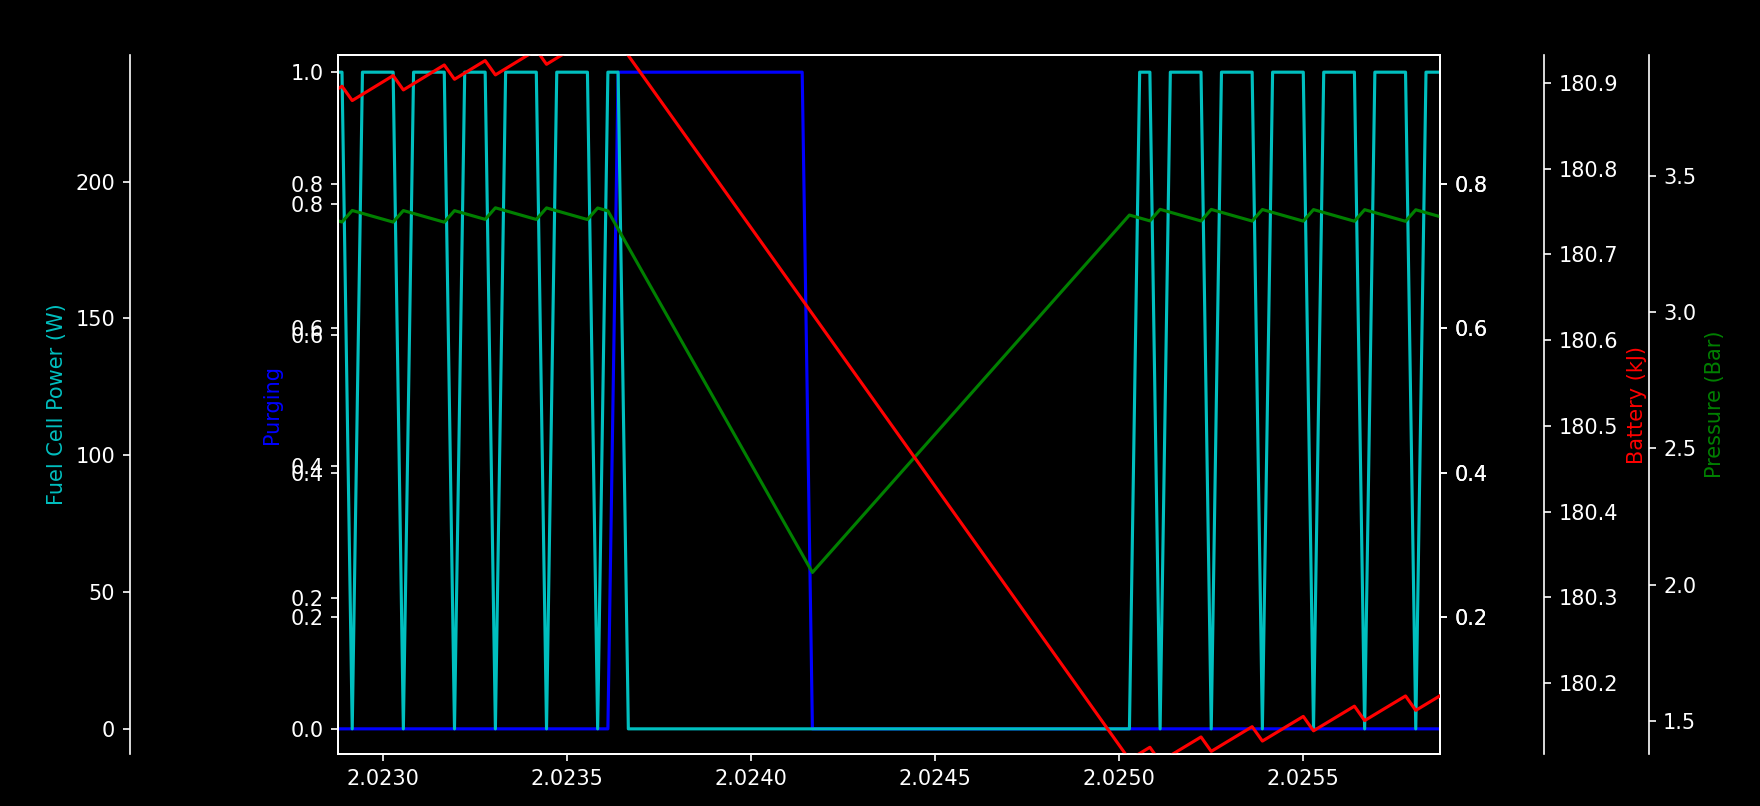
\includegraphics{media/simulated_purge.png}
        \caption{Simulated Purge Event}
        \label{fig:sim purge}
    \end{subfigure}
    \begin{subfigure}{\textwidth}
        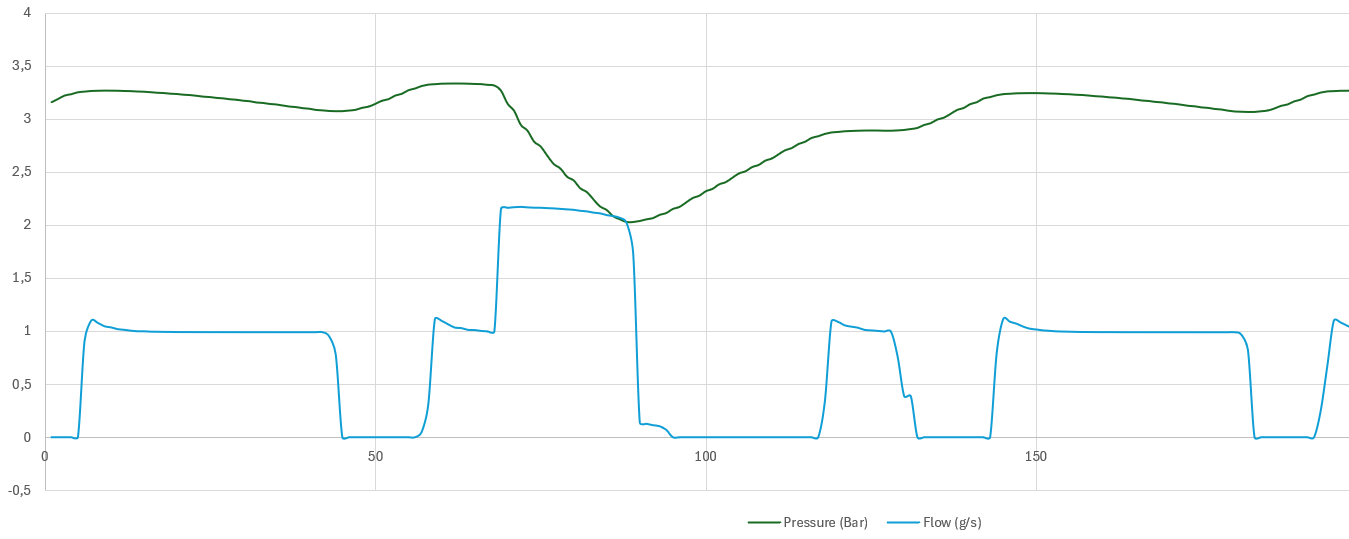
\includegraphics{media/air_purge.png}
        \caption{Measured Air Purge Event}
        \label{fig:air purge}
    \end{subfigure}
    \caption{Comparison of Simulation results with Compressed Air system}
    \label{fig:sim air comparison}
\end{figure}

\clearpage
%

\section{Hydrogen}
TBD

\clearpage
% \begin{xltabular}{\textwidth}{XllllX}
%     % header
%     \toprule
%     \textbf{Component}          & \textbf{Pin}         & \textbf{Connector}      & \textbf{Connects to}        & \textbf{Connector}      & \textbf{Wire}\\
%     \toprule
%     \endhead

%     % footer
%     \midrule
%     \multicolumn{6}{r}{\textit{Continued on next page...}}\\
%     \bottomrule
%     \endfoot

%     \bottomrule
%     \caption{Electrical Connections}
%     \label{tab:electrical connections}\\
%     \endlastfoot

%     % content
%     \multirow{2}{2cm}{Pressure Sensor}
%     & Vcc         & Attached wire  & 24V                & Terminal Block & Loose Wire\\
%     & Data        & Attached wire  & 4--20 mA Converter & Terminal Block & included\\
%     \midrule
%     \multirow{2}{2cm}{4--20 mA Converter}
%     & +           & Terminal block & Pressure Sensor    & Attached Wire  & included\\
%     & -           & Terminal block & GND                & Terminal Block & Loose Wire\\
%     & Analog Volt & DuPont (f)     & ADC                & DuPont (m)     & included\\
%     \midrule
%     ADC
%     & Analog Volt & DuPont (m)     & 4--20 mA Converter & DuPont (f)     & included\\
%     & Analog Volt & DuPont (m)     & Battery            & JST-XH~7 (f)   & JST-XH~7 (m) -- DuPont (m) DuPont (ff)\\
%     & Analog Volt & DuPont (m)     & ---                &                & \\
%     & Analog Volt & DuPont (m)     & ---                &                & \\
%     & \iic        & DuPont (f)     & \iic~Bus           & DuPont (m)     & included\\
%     \midrule
%     \iic~Bus
%     & \iic        & DuPont (m)     & ADC                & DuPont (f)     & included\\
%     & \iic        & DuPont (m)     & Power Meter        & DuPont (m)     & DuPont (ff)\\
%     & \iic        & DuPont (m)     & Power Meter        & DuPont (m)     & DuPont (ff)\\
%     & \iic        & DuPont (m)     & Power Meter        & DuPont (m)     & DuPont (ff)\\
%     & \iic        & DuPont (m)     & ---                &                & \\
%     & \iic        & DuPont (m)     & ---                &                & \\
%     & \iic        & DuPont (m)     & ---                &                & \\
%     & \iic        & DuPont (m)     & ---                &                & \\
%     & \iic        & DuPont (f)     & Raspberry Pi       & DuPont (m)     & included\\
%     \midrule
%     Fuel Cell
%     & Power Out   & XT60 (f)       & Power Meter 1      & Terminal Block & XT60 (m-)\\
%     \midrule
%     \multirow{2}{2cm}{Power Meter 1}
%     & Power In    & Terminal Block & Fuel Cell          & XT60 (f)       & XT60 (m-)\\
%     & Power Out   & Terminal Block & Buck Converter 1   & Terminal Block & Loose Wire\\
%     & \iic        & DuPont (m)     & \iic~Bus           & DuPont (m)     & DuPont (ff)\\
%     \midrule
%     \multirow{2}{2cm}{Buck Converter 1}
%     & Power In    & Terminal Block & Power Meter 1      & Terminal Block & Loose Wire\\
%     & Power Out   & Terminal Block & Relay              & Terminal Block & Loose Wire\\
%     \midrule
%     Relay
%     & Common      & Terminal Block & Buck Converter 1   & Terminal Block & Loose Wire\\
%     & NO          & Terminal Block & 24V                & Terminal Block & Loose Wire\\
%     & Control     & PCB Hole       & Raspberry Pi       & DuPont (m)     & DuPont (mf)\\
%     \midrule
%     \multirow{3}{2cm}{Power Meter 2}
%     & Power In    & Terminal Block & Battery            & XT60 (f)       & XT60 (m-)\\
%     & Power Out   & Terminal Block & 24V                & Terminal Block & Loose Wire\\
%     & \iic        & DuPont (m)     & \iic~Bus           & DuPont (m)     & DuPont (ff)\\
%     \midrule
%     Battery
%     & Power       & XT60 (f)       & Power Meter 2      & Terminal Block & XT60 (m-)\\
%     & Balance Leads & JST-XH~7 (f) & ADC                & DuPont (m)     & JST-XH~7 (m) -- DuPont (m) DuPont (ff)\\
%     \midrule
%     \multirow{2}{2cm}{Power Meter 3}
%     & Power In    & Terminal Block & ESC                & Attached Wire  & included\\
%     & Power Out   & Terminal Block & 24V                & Terminal Block & Loose Wire\\
%     \midrule
%     ESC
%     & Power In    & Attached Wire  & Power Meter 3      & Terminal Block & included\\
%     & 3 Phase Out & BLDC Plug (f)  & BLDC               & BLDC Plug (m)  & included\\
%     & Throttle    & DuPont (f)     & Raspberry Pi       & DuPont (m)     & included\\
%     & BEC         & DuPont (f)     & ---                &                &\\
%     & Active Break& DuPont (f)     & ---                &                &\\
%     \midrule
%     BLDC
%     & 3 Phase In  & BLDC Plug (m)  & ESC                & BLDC Plug (f)  & included\\
%     \midrule
%     \multirow{2}{2cm}{Buck Converter 2}
%     & Power In    & Terminal Block & 24V                & Terminal Block & Loose Wire \\
%     & Power Out   & Terminal Block & Raspberry Pi       & DuPont (m)     & DuPont (f-)\\
%     \midrule
%     Raspberry Pi
%     & 5V In       & DuPont (m)     & Buck Converter 2   & Terminal Block & DuPont (f-)\\
%     & \iic        & DuPont (m)     & \iic~Bus           & DuPont (f)     & included\\
%     \midrule
%     24V Bus
%     & Power       & Terminal Block & Pressure Sensor    & Terminal Block & Loose Wire\\
%     & Power       & Terminal Block & Relay              & Terminal Block & Loose Wire\\
%     & Power       & Terminal Block & Power Meter 2      & Terminal Block & Loose Wire\\
%     & Power       & Terminal Block & Power Meter 3      & Terminal Block & Loose Wire\\
%     & Power       & Terminal Block & Buck Converter 2   & Terminal Block & Loose Wire\\
% \end{xltabular}

% \newpage
%


\chapter{Conclusion}
\newpage
The goal of the SHARP-PS project was to investigate the feasibility of a hydrogen fuel cell based power generation and feed system for extending the mission duration of unmanned aerial vehicles. More specifically, the project aimed to investigate whether Solid Flow's cool gas generator and Stellar Space Industries' flow control technology could be integrated into a hybrid fuel cell power architecture suitable for UAV applications.

To support this objective, a hydrogen-based power generation and feed architecture was designed, simulated, and partially validated using a compressed air equivalent system and a hydrogen test bench.



% Results
\subsection*{Results}
The simulation results demonstrated that the proposed hybrid fuel cell and battery architecture is capable of maintaining stable operation during varying mission phases and fuel cell purge events. The simulations further showed that temporary fuel cell shutdown during low buffer pressure conditions can successfully be compensated by the hybrid battery system.

The compressed air equivalent tests showed behaviour closely matching the simulation results. In both systems, purge events resulted in temporary pressure drops within the CGG buffer volume, after which the On-Off controller successfully restored pressure by temporarily limiting hydrogen consumption. These results demonstrate that the selected control strategy is capable of maintaining stable flow conditions using only the internal CGG buffer volume.

The hydrogen test bench successfully demonstrated the integration of the electrical power management system, load emulation system, and data acquisition architecture.
% Measurements from the test bench confirmed that the selected hybrid battery configuration is capable of decoupling transient load behaviour from the fuel cell dynamics.

Requirement validation showed that the majority of functional, interface, and safety requirements were either directly validated through testing or demonstrated using simulations, equivalent systems, and manufacturer data.



% Research Question
\subsection*{Research Question}
This thesis aimed to answer the following research question:

`To what extent is a hydrogen fuel cell based power generation and feed system that integrates Solid Flow's cool gas generator and Stellar Space Industries' flow control unit feasible for extending the mission time of UAVs'

Based on the performed analyses, simulations, and experimental validation, it can be concluded that such a system is technically feasible and shows strong potential for long-endurance UAV applications.

The performed work demonstrates that a hybrid fuel cell and battery architecture can successfully compensate for the dynamic limitations of a fuel cell and cool gas generator combination while maintaining stable operation during varying load conditions and purge events. Furthermore, the theoretical energy density advantages of hydrogen storage indicate significant potential for increasing UAV mission duration compared to conventional battery systems.

However, the feasibility of the complete system remains partially dependent on the final performance of Solid Flow's cool gas generator, particularly regarding volumetric hydrogen storage capacity and long-duration operation. In addition, full UAV integration and flight testing were outside the scope of this project and therefore remain subjects for future work.


% Limitations
\subsection*{Limitations}
Several limitations affected the scope of this project. Most notably, hydrogen was not available in time to perform integrated hydrogen testing before completion of this report. As a result, full validation of the integrated hydrogen power system could not yet be completed.

Additionally, the cool gas generator and Stellar Space Industries' flow control unit were both still under development during the execution of this project. Commercial off-the-shelf equivalents were therefore used to emulate their expected behaviour where necessary.

Environmental testing and flight testing were also outside the scope of this project. Consequently, the environmental and flight performance requirements remain unverified.

Despite these limitations, the developed simulation models, compressed air equivalent system, and hydrogen test bench provide a strong foundation for future validation and flight integration.


% Final conclusion
\subsection*{Final Conclusion}
This project successfully demonstrated the design methodology, subsystem integration strategy, and control principles required for a hydrogen fuel cell based UAV power generation and feed system.

The results obtained from simulation and subsystem testing indicate that the proposed hybrid architecture is capable of providing stable electrical power while managing the dynamic behaviour of hydrogen generation and fuel cell operation. The developed test bench furthermore provides a valuable platform for future hydrogen testing and continued development of the SHARP project.

Overall, the work performed during this thesis demonstrates that hydrogen fuel cell based power systems represent a promising solution for extending UAV endurance and provide a viable direction for future sustainable aviation technologies.
\newpage


\chapter{Recommendations}%
\label{chap:recommendations}%
\emph{This chapter presents recommendations for future work and continued development of the SHARP-PS power generation and feed system. Although the performed simulations, subsystem tests, and test bench development demonstrate the technical feasibility of the proposed architecture, several aspects of the system remain unvalidated or require further optimisation before practical UAV integration can be achieved. The recommendations presented in this chapter provide a roadmap for the continued development of hydrogen fuel cell based UAV propulsion systems within the SHARP project.}
\newpage

\section{Integrated Hydrogen Testing}
The highest priority recommendation following this project is to perform fully integrated hydrogen testing using the completed hydrogen test bench. Although the compressed air equivalent system successfully demonstrated the expected flow dynamics and control behaviour, the interaction between the actual hydrogen fuel cell and hydrogen supply system has not yet been experimentally validated.

Future hydrogen tests should focus on verifying the complete behaviour of the integrated system under representative operating conditions. Particular attention should be given to the hydrogen consumption of the fuel cell during both steady-state operation and purge events. The purge frequency and purge duration should be measured and compared against manufacturer specifications and simulation assumptions. In addition, the pressure dynamics inside the CGG buffer volume should be analysed to verify whether the proposed buffer volume is sufficient to sustain stable fuel cell operation during transient conditions.

The integrated hydrogen tests should also evaluate the interaction between the fuel cell and the hybrid battery system. Specifically, the ability of the battery to compensate for temporary fuel cell shutdowns and transient load peaks should be validated under realistic mission load profiles. The resulting measurements can subsequently be compared with the simulation results and compressed air equivalent tests to further validate the developed system models.

Successful completion of these tests would significantly increase the technology readiness level of the SHARP-PS architecture and provide confidence for future UAV integration.

\section{Integration of Final FCU and CGG Hardware}
During this project, commercial off-the-shelf components and equivalent systems were used to emulate the behaviour of both Stellar Space Industries’ flow control unit and Solid Flow’s cool gas generator. Although this approach enabled subsystem development and validation, the final system behaviour remains dependent on the characteristics of the actual SHARP hardware.

Future work should therefore focus on integrating the final versions of both the flow control unit and the cool gas generator into the hydrogen test bench. Particular attention should be given to the dynamic response of the flow control system, as this directly affects the stability of the fuel cell operation and the pressure regulation within the hydrogen buffer volume.

In addition, the final cool gas generator should be evaluated for hydrogen generation consistency, startup behaviour, shutdown behaviour, pressure stability, and total hydrogen capacity. Since the mission endurance requirement is highly dependent on the achievable hydrogen storage density of the CGG, validating the final CGG performance is essential for determining the practical feasibility of the complete UAV power system.

Integration of the final SHARP hardware would also allow verification of the assumptions used throughout the simulations and equivalent-system testing performed during this thesis.

% \section{Advanced Control System Development}
\section{Long-Duration Endurance Testing}
One of the primary motivations behind the SHARP project is the possibility of significantly extending UAV mission duration using hydrogen fuel cell technology. Although simulations indicate that the proposed architecture may achieve mission durations in the order of 13--16 hours, this has not yet been experimentally validated.

Future work should therefore include long-duration endurance tests using the integrated hydrogen test bench. These tests should simulate representative mission profiles over extended periods of time while continuously monitoring hydrogen consumption, battery behaviour, fuel cell output, and thermal conditions.

Long-duration testing is particularly important because several effects only become visible during prolonged operation. These include fuel cell degradation, changes in purge frequency, thermal drift, battery cycling behaviour, and cumulative efficiency losses. In addition, the stability of the control system over long operating periods should be verified.

The results of these endurance tests should subsequently be compared against equivalent battery-based UAV power systems to quantify the actual endurance improvement achieved by the hydrogen architecture.

Successful endurance testing would provide one of the strongest demonstrations of the feasibility and practical value of the SHARP concept.

\section{Environmental Validation}
Environmental validation was outside the scope of this thesis but remains essential before operational deployment of a hydrogen powered UAV system can be considered.

Future work should therefore include dedicated environmental testing of the integrated system. Environmental chamber testing should be performed to verify operation under low-temperature conditions representative of high-altitude flight. Reduced-pressure testing should also be performed to investigate fuel cell behaviour at operating altitudes up to 3 km.

In addition, the effects of varying humidity levels on fuel cell performance and water management should be investigated. Since PEM fuel cells are sensitive to membrane hydration conditions, humidity may significantly influence efficiency and long-term reliability.


\section{Mechanical Optimisation and Weight Reduction}
The hydrogen test bench developed during this project was primarily designed as a flexible experimental platform rather than an optimised flight-ready system. As a result, the current implementation contains significant opportunities for mechanical optimisation and weight reduction.

Future development should focus on reducing the total mass and volume of the system while maintaining safety and functionality. This may include reducing the amount of sensors, integrating the fuel cell controller and power system controller into a single board and designing light weight mounting solutions. Thermal management and vibration isolation should also be considered during future mechanical redesigns.

Optimising the system mass and packaging efficiency is especially important because the achievable endurance improvement of hydrogen powered UAV systems is strongly dependent on overall system weight.

\section{UAV Integration and Flight Testing}
Although the developed hydrogen test bench provides a representative ground-test environment, the final objective of the SHARP project remains integration into an operational UAV platform. Ground testing alone cannot fully reproduce the environmental and operational conditions encountered during real flight.

Future work should therefore focus on mechanical and electrical integration of the power generation and feed system into the Wren Aerospace UAV platform. This integration process should consider structural mounting, centre-of-gravity effects, vibration resistance, cooling airflow, and accessibility for maintenance and refuelling.

Following integration, progressive flight testing should be performed. Initial tests should focus on low-risk operation such as short low altitude cruise tests under controlled conditions before moving towards long-endurance missions.

Flight testing should evaluate the behaviour of the complete system during realistic manoeuvres, varying propulsion loads, changing environmental conditions, and communication with the flight controller. Particular attention should be given to the interaction between the fuel cell system and the UAV propulsion electronics during rapid throttle changes.

Successful flight integration would represent a major milestone in the SHARP project and significantly increase the technology readiness level of the developed hydrogen power architecture.

\newpage


\begin{appendices}
    % \section*{Appendix A --- Research Matrix}
% \addcontentsline{toc}{section}{Appendix A --- Research Matrix}
\chapter{Research Matrix}\label{app:Research Matrix}

\ResearchMatrix%

\newpage

\end{appendices}

\newpage
\bibliography{references}
\end{document}
